%!TEX program = xelatex
%%% Document Options %%%
\documentclass[
    12pt,
    a4paper,
    oneside
]{report}

% --- Packages Essentiels ---
\usepackage[utf8]{inputenc}
\usepackage[T1]{fontenc}
% --- Packages pour le multilingue (Français, Anglais) ---
\usepackage{fontspec}   % Requis pour XeLaTeX et les polices \usepackage{fontspec}
\usepackage{polyglossia}
\setmainlanguage{french}
\setotherlanguage{english}
\usepackage{graphicx}
\usepackage{geometry}
\usepackage{listings}
\usepackage{xcolor}
\usepackage{float}
\usepackage{booktabs}
\usepackage{caption}
\usepackage{hyperref}
\usepackage{longtable}
\usepackage{array}
\usepackage{enumitem}
\usepackage{setspace}
\usepackage{fancyhdr}
\usepackage{ragged2e}
\usepackage{colortbl}
\usepackage{rotating}
\usepackage{tikz} %<-- Package déplacé ici, dans le préambule.
\usepackage[skins]{tcolorbox}
\usepackage{multirow}
\usepackage{caption}
\usepackage{amsmath}
\usepackage{tocloft}

% --- Configuration pour la table des matières ---
% Ajoute le mot "Chapitre" avant le numéro
\renewcommand{\cftchappresnum}{Chapitre } 
% Ajoute un point et un espace après le numéro du chapitre
\cftsetindents{chapter}{0em}{6em}
\renewcommand{\cftchapaftersnum}{. }
\usepackage[backend=biber, style=numeric, sorting=none]{biblatex}
\addbibresource{Bibliography/Bibliography.bib}
% \usepackage{pdflscape}
% --- Géométrie de la page ---
\geometry{
    a4paper,
    top=3.5cm,
    bottom=4cm,
    left=2.5cm,
    right=2.5cm
}
\setlength{\footskip}{1.5cm}
\setlength{\headheight}{16pt} % Taille ajustée pour un en-tête simple

% --- Configuration Hyperref ---
\hypersetup{
    colorlinks=true,
    linkcolor=blue!60!black,
    filecolor=magenta!60!black,
    urlcolor=cyan!60!black,
    citecolor=green!60!black,
    pdftitle={Personal Behavior Anomaly Detection System (PBADS)},
    pdfauthor={EL ALAMI Mohamed Majd \& LANDRICHI Leila},
    pdfsubject={Rapport Projet fin d'année},
    pdfkeywords={Détection d'anomalies, Machine Learning, Microservices, Spring Boot, Kafka, PostgreSQL, Gemini AI}
}

% --- Configuration des légendes ---
\captionsetup[figure]{font=small, labelfont=bf, skip=10pt}
\captionsetup[table]{font=small, labelfont=bf, skip=10pt}
\captionsetup[longtable]{font=small, labelfont=bf, skip=10pt}
\setlength{\abovecaptionskip}{15pt}

% --- Configuration des tableaux ---
% Amélioration de la visibilité des bordures
\setlength{\arrayrulewidth}{0.5pt}
\renewcommand{\arraystretch}{1.2}

% --- Configuration des en-têtes et pieds de page pour tout le document ---
\pagestyle{fancy}
\fancyhf{}
% \fancyhead[L]{Rapport de stage} % En-tête gauche simplifié
\fancyhead[R]{\leftmark}
\renewcommand{\headrulewidth}{0.4pt}
\fancyfoot[C]{\thepage}
\renewcommand{\footrulewidth}{0pt}

\fancypagestyle{plain}{ % Style pour les débuts de chapitre
\fancyhf{}
% \fancyhead[L]{Rapport de stage}
\fancyhead[R]{\leftmark}
\renewcommand{\headrulewidth}{0.4pt}
\fancyfoot[C]{\thepage}
\renewcommand{\footrulewidth}{0pt}
}

\begin{document}

% Justification globale
\justifying
\setlength{\parindent}{0pt}
\setlength{\parskip}{0.5em}
\raggedbottom

% --- NOUVELLE PAGE DE GARDE ---
\begin{titlepage}
\thispagestyle{empty} % Aucune en-tête ni pied de page sur cette page

% Définition de la couleur de l'accent (vert profond)
\definecolor{mydeepgreen}{RGB}{16,94,50}

% Structure de la page avec TikZ pour les éléments graphiques
\begin{tikzpicture}[remember picture, overlay]
    % Barre verticale vert profond sur la gauche
    \fill[mydeepgreen] (current page.north west) rectangle ([xshift=1.2cm]current page.south west);

    % Logos en haut de page (centrés)
    \node[anchor=north, yshift=-1.5cm] at (current page.north) {
        
\includegraphics[height=2cm]{Figures/logo-emsi-honoris.jpg}
    };

    % Année universitaire en bas de page
    \node[anchor=south, yshift=1.5cm] at (current page.south) {
        \large\bfseries Année universitaire 2025/2026
    };
\end{tikzpicture}

% Contenu textuel de la page de garde
\begin{center}
    \hspace*{1.5cm} % Décalage pour ne pas superposer la barre
    \begin{minipage}[c][0.8\textheight][c]{\dimexpr\textwidth-1.5cm\relax}
        \centering
        \vspace*{3cm}
        {\LARGE\bfseries Rapport Projet fin d'année}\\[2cm]
        {\Large 5ème année Ingénierie Informatique et Réseaux}\\[1.5cm]
        {\large Sous le thème}\\[0.5cm]
        {\huge\bfseries Système de Détection d'Anomalies Comportementales Personnelles (PBADS)}\\[2cm]
        {\large Année universitaire 2025/2026}\\[3cm]
        \vfill
        \raggedright
        \large
        {\bfseries Réalisé par :}\\[0.5cm]
        EL ALAMI Mohamed Majd \& LANDRICHI Leila \\[1.5cm]
        {\bfseries Encadré par :}\\[0.5cm]
        Pr. Benyoussef Marwa \\
    \end{minipage}
\end{center}
\end{titlepage}
% --- PAGE POUR LES REMARQUES DE L'ENCADRANT ---
\cleardoublepage % Crée une nouvelle page bien distincte
\thispagestyle{empty}  % Applique un style de page simple (numéro en bas)


% Vous pouvez laisser cette page vide pour que l'encadrant puisse écrire.

% --- Début du contenu du rapport ---

% Dedication
\clearpage
\markboth{DÉDICACE}{DÉDICACE}
\chapter*{DÉDICACE}
\setlength{\parskip}{1em}
Nous dédions ce travail à toutes les personnes qui nous ont soutenues tout au long de ce projet.

À Pr. Benyoussef Marwa, notre encadrante pédagogique, pour son accompagnement attentif, ses conseils pertinents et son soutien constant tout au long de cette expérience enrichissante.

À l'École Marocaine des Sciences de l'Ingénieur (EMSI), pour la qualité de la formation dispensée et les opportunités offertes aux étudiants dans le cadre de leur développement professionnel.

À nos familles et à notre entourage, pour leur présence, leurs encouragements et leur soutien moral, qui nous ont permis de mener à bien ce projet.

\addcontentsline{toc}{chapter}{Dédicace}

% Acknowledgments
\clearpage
\markboth{REMERCIEMENTS}{REMERCIEMENTS}
\chapter*{REMERCIEMENTS}
\setlength{\parskip}{1em}
Nous tenons à exprimer notre profonde gratitude à toutes les personnes qui ont contribué à la réalisation de ce projet de fin d'année.

Nous adressons nos remerciements les plus sincères à Pr. Benyoussef Marwa, notre encadrante pédagogique à l'École Marocaine des Sciences de l'Ingénieur (EMSI), pour son expertise, sa disponibilité, ses précieux conseils et son accompagnement académique tout au long de ce projet. Sa guidance, sa bienveillance et ses orientations constructives ont été essentielles pour la réussite de ce travail.

Nous remercions également tous nos professeurs et encadrants de l'EMSI pour la qualité de leur enseignement et leur accompagnement tout au long de notre formation.

Enfin, merci à toutes celles et ceux qui, de près ou de loin, ont contribué à la réalisation de ce travail.

À tous… merci.
\addcontentsline{toc}{chapter}{Remerciements}

% Acknowledgments (English)
\clearpage
\markboth{ACKNOWLEDGMENTS}{ACKNOWLEDGMENTS}
\chapter*{ACKNOWLEDGMENTS}
\setlength{\parskip}{1em}
We would like to express our deep gratitude to everyone who contributed to the completion of this end-of-year project.

Our sincere thanks go to Pr. Benyoussef Marwa, our academic supervisor at the Moroccan School of Engineering Sciences (EMSI), for her expertise, availability, and valuable guidance. Her support and constructive feedback were essential throughout this experience.

We would also like to thank all our professors and academic mentors at EMSI for the quality of education and the support they have provided throughout our studies.

Finally, thank you to everyone who, directly or indirectly, contributed to the development of this project.

To all… thank you.

\addcontentsline{toc}{chapter}{Acknowledgments}


% Abstract (French)
\clearpage
\markboth{RÉSUMÉ}{RÉSUMÉ}
\chapter*{Résumé}
Ce travail présente la conception et la réalisation d'un \textbf{Système de Détection d'Anomalies Comportementales Personnelles (PBADS)} basé sur une architecture microservices. Le système analyse les données quotidiennes des utilisateurs (sommeil, activité physique, alimentation, humeur) et détecte en temps réel les anomalies comportementales à l'aide d'algorithmes d'apprentissage automatique non supervisés.

La solution repose sur une \textbf{architecture microservices} avec 13 services distincts, incluant un service d'authentification (JWT), un service de données, un service de modèles ML, un service d'inférence pour la détection d'anomalies, un service d'alertes, et un service de recommandations alimenté par Google Gemini AI. La communication entre services utilise Kafka pour la messagerie asynchrone et HTTP/REST pour les appels synchrones, avec un mécanisme de fallback pour garantir la résilience.

Le modèle de données structure les entités principales : \texttt{User}, \texttt{DailyData}, \texttt{Alert} et \texttt{Recommendation}. Le système utilise des algorithmes de détection d'anomalies (Isolation Forest et One-Class SVM) pour identifier les écarts par rapport aux comportements normaux, génère des alertes avec des niveaux de sévérité (NORMAL, LOW, MEDIUM, HIGH), et fournit des recommandations personnalisées via l'intégration avec Google Gemini AI.

Les bénéfices observés : \textbf{détection automatique des anomalies}, \textbf{recommandations personnalisées}, \textbf{notifications en temps réel}, et \textbf{visualisation interactive} des données comportementales via un tableau de bord avec filtres temporels. Le système offre une scalabilité élevée grâce à l'architecture microservices et une tolérance aux pannes via Resilience4j.

\textbf{Mots-clés :} Détection d'anomalies, Machine Learning, Microservices, Spring Boot, Kafka, PostgreSQL, Isolation Forest, One-Class SVM, Google Gemini AI, Recommandations personnalisées, Architecture microservices.

\addcontentsline{toc}{chapter}{Résumé}

% Abstract (English)
\clearpage
\markboth{ABSTRACT}{ABSTRACT}
\chapter*{Abstract}
This work presents the design and implementation of a \textbf{Personal Behavior Anomaly Detection System (PBADS)} based on a microservices architecture. The system analyzes users' daily data (sleep, physical activity, diet, mood) and detects behavioral anomalies in real-time using unsupervised machine learning algorithms.

The solution is built on a \textbf{microservices architecture} with 13 distinct services, including an authentication service (JWT), a data service, an ML model service, an inference service for anomaly detection, an alert service, and a recommendation service powered by Google Gemini AI. Inter-service communication uses Kafka for asynchronous messaging and HTTP/REST for synchronous calls, with a fallback mechanism to ensure resilience.

The data model structures the main entities: \textit{User}, \textit{DailyData}, \textit{Alert} and \textit{Recommendation}. The system uses anomaly detection algorithms (Isolation Forest and One-Class SVM) to identify deviations from normal behaviors, generates alerts with severity levels (NORMAL, LOW, MEDIUM, HIGH), and provides personalized recommendations through integration with Google Gemini AI.

The observed benefits include: \textbf{automatic anomaly detection}, \textbf{personalized recommendations}, \textbf{real-time notifications}, and \textbf{interactive visualization} of behavioral data through a dashboard with temporal filters. The system offers high scalability through the microservices architecture and fault tolerance via Resilience4j.

\textbf{Keywords:} Anomaly Detection, Machine Learning, Microservices, Spring Boot, Kafka, PostgreSQL, Isolation Forest, One-Class SVM, Google Gemini AI, Personalized Recommendations, Microservices Architecture.

\addcontentsline{toc}{chapter}{Abstract}

% --- Table des matières ---
\clearpage
% On s'assure que l'en-tête de la ToC est correct jusqu'au bout
\markboth{TABLE DES MATIÈRES}{TABLE DES MATIÈRES} 
\tableofcontents
\addcontentsline{toc}{chapter}{Table des matières}

% --- Liste des figures ---
\clearpage
\markboth{LISTE DES FIGURES}{LISTE DES FIGURES}
\listoffigures
\addcontentsline{toc}{chapter}{Liste des Figures}

% --- Liste des tableaux ---
\clearpage
\markboth{LISTE DES TABLEAUX}{LISTE DES TABLEAUX}
\listoftables
\addcontentsline{toc}{chapter}{Liste des Tableaux}
% Définition de la couleur pour les titres et résumés de chapitre
\definecolor{chapterblue}{RGB}{60, 90, 120} % Une couleur bleu-gris foncé

% --- NOUVEAU CODE (CORRIGÉ) ---

% Commande pour les pages de titre de chapitre SANS numéro (ex: Introduction)
\newcommand{\chaptertitlepagenonum}[1]{
  \clearpage
  \addcontentsline{toc}{chapter}{#1}
  \thispagestyle{plain}
  \markboth{#1}{}
  \begingroup % On ouvre un groupe pour contenir l'effet de \raggedright
  \raggedright % Aligner à gauche
  \vspace*{0.20\textheight}
  {\fontsize{28}{34}\selectfont\color{chapterblue}\bfseries #1\par}
  \vspace*{2cm}
  \endgroup % On ferme le groupe, la justification redevient la norme
}

% Commande pour les pages de titre de chapitre AVEC numéro
\newcommand{\chaptertitlepage}[1]{
  \clearpage
  \refstepcounter{chapter}
  \addcontentsline{toc}{chapter}{\protect\numberline{\thechapter}#1}
  \thispagestyle{plain}
  \markboth{\chaptername\ \thechapter: #1}{#1}
  \begingroup % On ouvre un groupe pour contenir l'effet de \raggedright
  \raggedright % Aligner à gauche
  \vspace*{0.20\textheight}
  {\fontsize{28}{34}\selectfont\color{chapterblue}\bfseries Chapitre \thechapter{} : #1\par}
  \vspace*{2cm}
  \endgroup % On ferme le groupe, la justification redevient la norme
}
% --- Liste des abréviations (SOLUTION DÉFINITIVE) ---
\clearpage
% ÉTAPE 1: On modifie l'en-tête pour les pages standards ('fancy')
\fancyhead[R]{LISTE DES ABRÉVIATIONS}

% ÉTAPE 2: On modifie AUSSI l'en-tête pour la PREMIÈRE page du chapitre ('plain')
\fancypagestyle{plain}{
    \fancyhf{}
    % \fancyhead[L]{Rapport de stage}
    \fancyhead[R]{LISTE DES ABRÉVIATIONS} % <-- Modification cruciale ici
    \renewcommand{\headrulewidth}{0.4pt}
    \fancyfoot[C]{\thepage}
    \renewcommand{\footrulewidth}{0pt}
}

% Maintenant que les DEUX styles sont prêts, on peut lancer le chapitre.
\chapter*{Liste des abréviations}
% !TEX root = ../IPLeiriaMain.tex

% On utilise l'environnement "center" pour contenir l'effet de centrage
% et s'assurer qu'il n'affecte pas le reste du document.
\begin{center}
    \begin{longtable}{|p{3.5cm}|p{11.5cm}|}
        
        % Ligne horizontale en haut du tableau
        \hline
        
        % En-têtes des colonnes en gras
        \textbf{Abréviation} & \textbf{Description} \\
        
        % Ligne horizontale sous les en-têtes
        \hline
        \endfirsthead % Fin de l'en-tête pour la première page
        
        % En-tête pour les pages suivantes (si le tableau continue)
        \hline
        \textbf{Abréviation} & \textbf{Description} \\
        \hline
        \endhead
        
        % Ligne de fin pour chaque page
        \hline
        \endfoot
        
        % Ligne finale en bas du tableau
        \hline
        \endlastfoot
    
        % Contenu du tableau, avec une ligne horizontale après chaque entrée
        API & Application Programming Interface (Interface de Programmation d'Application). \\
        \hline
        PBADS & Personal Behavior Anomaly Detection System (Système de Détection d'Anomalies Comportementales Personnelles). \\
        \hline
        ML & Machine Learning (Apprentissage Automatique). \\
        \hline
        AI & Artificial Intelligence (Intelligence Artificielle). \\
        \hline
        JWT & JSON Web Token (Jeton d'authentification basé sur JSON). \\
        \hline
        CRUD & Create, Read, Update, Delete (Créer, Lire, Mettre à jour, Supprimer). \\
        \hline
        DB & Database (Base de Données). \\
        \hline
        EMSI & École Marocaine des Sciences de l'Ingénieur. \\
        \hline
        JPA & Java Persistence API (utilisé via Spring Data JPA pour l'accès et la gestion des données). \\
        \hline
        REST & Representational State Transfer, style architectural pour les APIs exposées par le backend. \\
        \hline
        PostgreSQL & Système de gestion de base de données relationnelle utilisé pour stocker les données. \\
        \hline
        Spring Boot & Framework Java pour le développement backend de l'application. \\
        \hline
        Spring Cloud & Suite d'outils pour le développement d'applications microservices. \\
        \hline
        Eureka & Service de découverte et registre des microservices (Spring Cloud Netflix Eureka). \\
        \hline
        Kafka & Apache Kafka, broker de messagerie distribué pour la communication asynchrone entre services. \\
        \hline
        Thymeleaf & Moteur de template côté serveur pour le rendu des pages HTML. \\
        \hline
        Chart.js & Bibliothèque JavaScript pour la création de graphiques interactifs. \\
        \hline
        UI / UX & User Interface / User Experience (Interface Utilisateur / Expérience Utilisateur). \\
        \hline
        UML & Unified Modeling Language (Langage de Modélisation Unifié), utilisé pour la modélisation du système. \\
        \hline
        Isolation Forest & Algorithme d'apprentissage automatique non supervisé pour la détection d'anomalies. \\
        \hline
        One-Class SVM & Support Vector Machine à une classe, algorithme alternatif pour la détection d'anomalies. \\
        \hline
        MLflow & Plateforme open-source pour la gestion du cycle de vie du machine learning. \\
        \hline
        scikit-learn & Bibliothèque Python pour l'apprentissage automatique. \\
        \hline
        Gemini AI & Modèle d'intelligence artificielle de Google utilisé pour la génération de recommandations. \\
        \hline
        Resilience4j & Bibliothèque Java pour la tolérance aux pannes (circuit breaker, retry, fallback). \\
        \hline
        BCrypt & Algorithme de hachage de mot de passe utilisé pour la sécurité. \\
        \hline
        Redis & Système de stockage clé-valeur en mémoire utilisé pour le cache et la gestion de session. \\
        \hline
        Prometheus & Système de surveillance et d'alerte open-source pour les métriques. \\
        \hline
        Grafana & Plateforme open-source de visualisation et d'analyse de métriques. \\
        \hline
        HTTP & HyperText Transfer Protocol (Protocole de Transfert HyperTexte). \\
        \hline
        JSON & JavaScript Object Notation (Format de données structuré). \\
        \hline
        CSV & Comma-Separated Values (Valeurs séparées par des virgules). \\
        \hline
        Maven & Outil de gestion et d'automatisation de projets Java. \\
        \hline
        dotenv-java & Bibliothèque Java pour le chargement de variables d'environnement depuis des fichiers .env. \\
        \hline
        WebFlux & Framework réactif de Spring pour les applications non-bloquantes. \\
        \hline
        OpenFeign & Client HTTP déclaratif pour la communication entre microservices (Spring Cloud OpenFeign). \\
        \hline
    
    \end{longtable}
\end{center}

\addcontentsline{toc}{chapter}{Liste des abréviations}

% --- Restauration du comportement normal pour TOUT le reste du document ---
\clearpage
% ÉTAPE 3: On restaure l'en-tête pour les pages standards ('fancy')
\fancyhead[R]{\leftmark}

% ÉTAPE 4: On restaure l'en-tête pour les premières pages de chapitre ('plain')
\fancypagestyle{plain}{
    \fancyhf{}
    % \fancyhead[L]{Rapport de stage}
    \fancyhead[R]{\leftmark} % <-- On remet la version automatique
    \renewcommand{\headrulewidth}{0.4pt}
    \fancyfoot[C]{\thepage}
    \renewcommand{\footrulewidth}{0pt}
}
\chaptertitlepagenonum{Introduction générale}
% Résumé pour l'Introduction générale
% \begin{flushright}
% \begin{minipage}{0.6\textwidth}
% Ce rapport documente notre projet de fin d'année, axé sur le développement d'un système de détection d'anomalies comportementales personnelles (PBADS). Face aux défis croissants de l'analyse des comportements quotidiens et de l'amélioration de la qualité de vie, notre objectif est de proposer une solution innovante basée sur l'apprentissage automatique et l'intelligence artificielle. Nous détaillerons dans les chapitres suivants l'approche méthodologique, les choix techniques, la conception et l'implémentation de notre solution microservices.
% \end{minipage}
% \end{flushright}
\clearpage
Dans le contexte actuel de transformation digitale et de prise de conscience croissante de l'importance de la santé et du bien-être personnel, la capacité à analyser et comprendre nos comportements quotidiens représente un enjeu majeur. Les habitudes de vie telles que le sommeil, l'activité physique, l'alimentation, l'hydratation, le temps d'étude et l'humeur influencent significativement notre qualité de vie et notre performance. Cependant, identifier les anomalies dans ces comportements et comprendre leurs causes reste un défi complexe nécessitant des outils avancés d'analyse de données et d'intelligence artificielle.

Pour répondre à ces enjeux, nous avons conçu et réalisé le \textbf{Personal Behavior Anomaly Detection System (PBADS)}, un système complet de détection d'anomalies comportementales basé sur une architecture microservices. Cette solution intégrée traite les données quotidiennes des utilisateurs depuis leur saisie jusqu'à la génération d'alertes et de recommandations personnalisées, en passant par l'analyse en temps réel à l'aide d'algorithmes d'apprentissage automatique non supervisés.

L'architecture technique de la solution repose sur une approche moderne et robuste. Le système suit une \textbf{architecture microservices} avec 13 services distincts, permettant une séparation claire des responsabilités, une scalabilité élevée et une tolérance aux pannes. Le backend s'appuie sur le framework \textbf{Spring Boot} qui fournit des APIs REST complètes, un système de sécurité avancé basé sur JWT pour l'authentification et l'autorisation, ainsi qu'une intégration avec Kafka pour la communication asynchrone entre services. Le frontend utilise \textbf{Thymeleaf} avec Spring MVC pour le rendu côté serveur, \textbf{Chart.js} pour la visualisation interactive des données, et un système de notifications push en temps réel. Le modèle de données structure de manière cohérente les entités clés du système : \texttt{User} pour la gestion des utilisateurs, \texttt{DailyData} pour les données quotidiennes, \texttt{Alert} pour les alertes générées, et \texttt{Recommendation} pour les recommandations générées par l'IA.

La détection d'anomalies constitue le cœur du système, utilisant des algorithmes d'apprentissage automatique non supervisés (\textbf{Isolation Forest} et \textbf{One-Class SVM}) pour identifier les écarts par rapport aux comportements normaux sans nécessiter de données étiquetées. Le système calcule un score d'anomalie (0-1) et détermine un niveau de sévérité (NORMAL, LOW, MEDIUM, HIGH) pour chaque entrée de données. Lorsqu'une anomalie est détectée, le système génère automatiquement une alerte et sollicite le \textbf{service de recommandations} alimenté par \textbf{Google Gemini AI} pour produire des suggestions personnalisées visant à améliorer les habitudes de l'utilisateur.

La méthodologie de développement a suivi une approche agile avec une planification structurée en sprints, permettant une adaptation rapide aux besoins évolutifs et une livraison incrémentale des fonctionnalités. Cette approche s'est traduite par une priorisation continue des fonctionnalités, des itérations courtes permettant une validation régulière, et des revues régulières pour ajuster les orientations.

Ce rapport technique documente l'ensemble du projet PBADS, couvrant de manière exhaustive le contexte et les objectifs du projet, l'architecture microservices mise en place, la modélisation des données et des processus avec les diagrammes UML, l'implémentation détaillée des microservices, les algorithmes de machine learning utilisés, l'intégration avec Google Gemini AI, et les résultats obtenus. Le document met en évidence les apports concrets de la solution : détection automatique des anomalies comportementales, génération de recommandations personnalisées, notifications en temps réel, et visualisation interactive des données via un tableau de bord moderne avec filtres temporels.

\vspace{1cm}

\textbf{Mots-clés :} Détection d'anomalies, Machine Learning, Microservices, Spring Boot, Kafka, PostgreSQL, Isolation Forest, One-Class SVM, Google Gemini AI, Recommandations personnalisées, Architecture microservices, Thymeleaf, Chart.js, Resilience4j.


% --- Chapter 1 ---
\chaptertitlepage{Contexte général et planification du projet}
% Résumé pour la page de titre du chapitre 1
\begin{flushright}
\begin{minipage}{0.6\textwidth}
Ce chapitre établit les fondations du projet PBADS en détaillant le contexte général et les problématiques spécifiques liées à la détection d'anomalies comportementales. Nous y exposerons les objectifs clairs du projet, la méthodologie de développement agile choisie, et le plan de travail détaillé. Une analyse des besoins utilisateurs et une stratégie d'architecture microservices seront également abordées pour garantir une exécution robuste et une scalabilité élevée.
\end{minipage}
\end{flushright}
\clearpage
\section{Introduction}
Ce chapitre présente le contexte et la problématique du \textbf{Personal Behavior Anomaly Detection System (PBADS)}, un système de détection d'anomalies comportementales conçu pour analyser les habitudes quotidiennes des utilisateurs et identifier les écarts par rapport aux comportements normaux. Cette solution technologique a été développée pour répondre au besoin croissant d'outils intelligents permettant de comprendre et d'améliorer nos modes de vie à travers l'analyse de données comportementales et la génération de recommandations personnalisées.

\section{Contexte général}

\subsection{Environnement et motivation}
Dans un monde où la santé et le bien-être personnel deviennent des priorités croissantes, la capacité à suivre et analyser nos comportements quotidiens représente un enjeu majeur. Les habitudes de vie telles que la qualité du sommeil, le niveau d'activité physique, l'alimentation, l'hydratation, le temps consacré à l'étude ou au travail, et l'état émotionnel influencent significativement notre santé physique et mentale, notre productivité et notre qualité de vie globale.

Cependant, identifier les anomalies dans ces comportements et comprendre leurs causes reste un défi complexe. Les méthodes traditionnelles d'auto-évaluation sont souvent subjectives et peu fiables, tandis que l'analyse manuelle de grandes quantités de données comportementales est fastidieuse et sujette à l'erreur humaine. Il existe donc un besoin réel d'outils automatisés capables de détecter les anomalies comportementales de manière objective, de fournir des insights actionnables, et de générer des recommandations personnalisées pour améliorer les habitudes de vie.

\subsection{Situation initiale et problématique}
Avant le développement de PBADS, l'analyse des comportements personnels reposait principalement sur des méthodes manuelles et fragmentées. Les utilisateurs devaient consigner leurs données quotidiennes dans des tableurs Excel ou des applications mobiles isolées, sans capacité d'analyse approfondie ni de détection automatique des anomalies. Cette approche présentait plusieurs limitations critiques :

\textbf{Limitations observées :}

\begin{itemize}
    \item \textbf{Absence de détection automatique :} Les utilisateurs devaient identifier manuellement les anomalies dans leurs données, ce qui est subjectif et peu fiable, surtout pour des patterns complexes ou subtils.
    \item \textbf{Manque d'analyse prédictive :} Aucun système ne permettait d'anticiper les tendances comportementales ou d'identifier les facteurs contribuant aux anomalies.
    \item \textbf{Recommandations génériques :} Les conseils fournis étaient souvent génériques et non adaptés au profil spécifique de chaque utilisateur.
    \item \textbf{Fragmentation des données :} Les données étaient dispersées dans différents outils sans vue d'ensemble cohérente.
    \item \textbf{Absence de notifications proactives :} Les utilisateurs n'étaient pas alertés en temps réel des anomalies détectées.
    \item \textbf{Manque de visualisation interactive :} Les outils existants offraient peu de capacités de visualisation et de filtrage temporel des données.
\end{itemize}

\subsection{Objectif de la solution}
L'objectif principal est de fournir un \textbf{système intégré de détection d'anomalies comportementales} qui automatise l'analyse des données quotidiennes des utilisateurs et génère des insights actionnables. La solution PBADS doit permettre :

\begin{itemize}
    \item \textbf{Saisie structurée des données quotidiennes :} Interface intuitive pour enregistrer les habitudes de vie (sommeil, activité physique, alimentation, hydratation, étude, humeur).
    \item \textbf{Détection automatique des anomalies :} Utilisation d'algorithmes d'apprentissage automatique non supervisés (Isolation Forest, One-Class SVM) pour identifier les écarts par rapport aux comportements normaux sans nécessiter de données étiquetées.
    \item \textbf{Classification des anomalies :} Attribution d'un score d'anomalie (0-1) et d'un niveau de sévérité (NORMAL, LOW, MEDIUM, HIGH) pour chaque détection.
    \item \textbf{Génération d'alertes intelligentes :} Création automatique d'alertes avec identification des facteurs contribuant à l'anomalie.
    \item \textbf{Recommandations personnalisées :} Intégration avec Google Gemini AI pour générer des suggestions adaptées au profil et aux habitudes spécifiques de chaque utilisateur.
    \item \textbf{Visualisation interactive :} Tableau de bord moderne avec graphiques interactifs (Chart.js) et filtres temporels (semaine, mois, année, tout).
    \item \textbf{Notifications en temps réel :} Système de notifications push (toast) pour alerter les utilisateurs immédiatement lorsqu'une nouvelle anomalie est détectée.
    \item \textbf{Gestion des utilisateurs :} Interface d'administration pour la gestion des comptes utilisateurs avec contrôle d'accès basé sur les rôles (ADMIN, USER).
\end{itemize}

\subsection{Architecture microservices}
Pour répondre à ces objectifs, PBADS suit une \textbf{architecture microservices} avec 13 services distincts, permettant une séparation claire des responsabilités, une scalabilité élevée et une tolérance aux pannes. Cette architecture comprend :

\begin{itemize}
    \item \textbf{Couche Frontend :} Service frontend (Thymeleaf) pour l'interface utilisateur
    \item \textbf{Couche API Gateway :} Point d'entrée unique pour toutes les requêtes client
    \item \textbf{Couche Infrastructure :} Eureka (découverte de services), Config Server (configuration centralisée), Kafka (messagerie asynchrone), PostgreSQL (bases de données), Redis (cache), MLflow (gestion des modèles ML)
    \item \textbf{Couche Services Métier :} Auth Service, Data Service, Model Service, Inference Service, Alert Service, Monitoring Service, Recommendation Service
\end{itemize}

La communication entre services utilise Kafka pour la messagerie asynchrone et HTTP/REST pour les appels synchrones, avec un mécanisme de fallback pour garantir la résilience en cas de panne de Kafka.

\section{Conclusion}
Ce chapitre a présenté le contexte et les motivations derrière le développement du système PBADS. L'analyse de la situation existante a révélé des lacunes significatives en termes de détection automatique des anomalies, d'analyse prédictive, et de génération de recommandations personnalisées. Ces constats ont motivé le développement d'une solution intégrée basée sur une architecture microservices qui automatise l'analyse des comportements quotidiens et fournit des insights actionnables pour améliorer la qualité de vie des utilisateurs. La méthodologie de développement agile et la planification structurée permettront de répondre efficacement aux enjeux de détection d'anomalies, de personnalisation des recommandations, et de scalabilité du système.


% --- Chapter 2 ---
\chaptertitlepage{Modélisation}
% Résumé pour la page de titre du chapitre 2
\begin{flushright}
\begin{minipage}{0.6\textwidth}
Ce chapitre présente la modélisation complète du système PBADS, incluant l'analyse des besoins utilisateurs, la définition des objectifs, la méthodologie agile adoptée, et la modélisation conceptuelle avec les diagrammes UML (cas d'utilisation, classes, séquences). L'étude des lacunes des solutions existantes a permis d'identifier les besoins critiques en matière de détection automatique d'anomalies, de génération de recommandations personnalisées, et de visualisation interactive des données.
\end{minipage}
\end{flushright}
\clearpage
Ce chapitre présente la modélisation complète du système PBADS, incluant l'analyse des besoins, la définition des objectifs, la méthodologie adoptée, et la modélisation conceptuelle avec les diagrammes UML.

\section{Modélisation du système}

Cette section présente les diagrammes de modélisation qui illustrent l'architecture et les interactions du système PBADS.

\subsection{Contexte général}

\subsubsection{Situation actuelle et pratique existante}

Avant le développement de PBADS, l'analyse des comportements personnels reposait principalement sur des méthodes manuelles et fragmentées. Les utilisateurs devaient consigner leurs données quotidiennes dans des tableurs Excel ou des applications mobiles isolées, sans capacité d'analyse approfondie ni de détection automatique des anomalies.

\textbf{Lacunes identifiées dans les solutions existantes :}

\begin{itemize}
    \item \textbf{Absence de détection automatique :} Les utilisateurs devaient identifier manuellement les anomalies dans leurs données, ce qui est subjectif et peu fiable.
    \item \textbf{Manque d'analyse prédictive :} Aucun système ne permettait d'anticiper les tendances comportementales ou d'identifier les facteurs contribuant aux anomalies.
    \item \textbf{Recommandations génériques :} Les conseils fournis étaient souvent génériques et non adaptés au profil spécifique de chaque utilisateur.
    \item \textbf{Fragmentation des données :} Les données étaient dispersées dans différents outils sans vue d'ensemble cohérente.
    \item \textbf{Absence de notifications proactives :} Les utilisateurs n'étaient pas alertés en temps réel des anomalies détectées.
    \item \textbf{Manque de visualisation interactive :} Les outils existants offraient peu de capacités de visualisation et de filtrage temporel des données.
\end{itemize}

\textbf{Objectif de la solution}

L'objectif principal est de fournir un système intégré de détection d'anomalies comportementales qui automatise l'analyse des données quotidiennes des utilisateurs et génère des insights actionnables. La solution PBADS doit permettre la saisie structurée des données quotidiennes, la détection automatique des anomalies à l'aide d'algorithmes d'apprentissage automatique non supervisés, la génération d'alertes intelligentes avec identification des facteurs contribuant à l'anomalie, et la production de recommandations personnalisées via l'intégration avec Google Gemini AI.

\subsection{Enjeux et objectifs}

Les enjeux majeurs de PBADS sont : détection automatique des anomalies comportementales, génération de recommandations personnalisées, notifications en temps réel, et visualisation interactive des données. Ces enjeux se traduisent par les objectifs concrets suivants :

\begin{itemize}
    \item \textbf{Gestion des données quotidiennes :} Saisie structurée des habitudes de vie (sommeil, activité physique, alimentation, hydratation, étude, humeur).
    \item \textbf{Détection automatique d'anomalies :} Utilisation d'algorithmes ML (Isolation Forest, One-Class SVM) pour identifier les écarts par rapport aux comportements normaux.
    \item \textbf{Génération d'alertes intelligentes :} Création automatique d'alertes avec niveaux de sévérité (NORMAL, LOW, MEDIUM, HIGH) et facteurs contribuant à l'anomalie.
    \item \textbf{Recommandations personnalisées :} Intégration avec Google Gemini AI pour générer des suggestions adaptées au profil de chaque utilisateur.
    \item \textbf{Visualisation interactive :} Tableau de bord avec graphiques interactifs (Chart.js) et filtres temporels (semaine, mois, année, tout).
    \item \textbf{Notifications en temps réel :} Système de notifications push (toast) pour alerter les utilisateurs immédiatement.
    \item \textbf{Gestion des utilisateurs :} Interface d'administration pour la gestion des comptes avec contrôle d'accès basé sur les rôles (ADMIN, USER).
\end{itemize}

\subsection{Méthodologie adoptée}

Pour ce projet, nous avons opté pour une méthodologie agile, qui favorise un développement itératif et incrémental. Chaque itération permet de livrer des fonctionnalités prêtes à l'usage tout en recueillant régulièrement des retours des utilisateurs.

\textbf{Le cycle de vie du projet}

Le cycle de vie de notre projet comprend les activités suivantes :

\begin{enumerate}
    \item \textbf{Analyse des besoins et faisabilité :} Identification des besoins fonctionnels et non fonctionnels pour la détection d'anomalies comportementales.
    \item \textbf{Planification et priorisation :} Création du backlog produit, définition des priorités et planification des itérations.
    \item \textbf{Conception :} Élaboration des spécifications de l'architecture microservices, des bases de données et des interfaces utilisateur.
    \item \textbf{Développement :} Implémentation progressive des microservices avec des revues de code et une intégration continue.
    \item \textbf{Tests :} Vérification de chaque fonctionnalité par des tests unitaires, fonctionnels et d'intégration.
    \item \textbf{Documentation :} Rédaction des informations nécessaires à l'utilisation, la maintenance et les futures évolutions.
    \item \textbf{Livraison et déploiement :} Livraison progressive des incréments et mise en production du système.
\end{enumerate}

Cette approche agile assure une meilleure collaboration entre les parties prenantes et une flexibilité accrue face aux changements, tout en maintenant un haut niveau de qualité.

\section{Étude Conceptuelle}

Cette section présente l'étude conceptuelle du système avec les diagrammes UML qui modélisent les interactions et la structure de la solution PBADS.

\subsection{Méthodologie}

L'étude conceptuelle suit une approche structurée basée sur l'analyse des besoins utilisateurs et la modélisation des interactions système. Cette méthodologie permet de capturer les exigences fonctionnelles et non-fonctionnelles, d'identifier les acteurs clés, et de concevoir une architecture cohérente et évolutive.

\subsection{Les acteurs principaux}

Le système PBADS implique plusieurs acteurs aux rôles et responsabilités distincts. Le tableau suivant présente l'ensemble des acteurs identifiés avec leurs fonctionnalités principales.

\begin{table}[H]
\centering
\small
\renewcommand{\arraystretch}{1.3}
\begin{tabular}{|p{3cm}|p{4.5cm}|p{6.5cm}|}
\hline
\textbf{Acteur} & \textbf{Rôle} & \textbf{Fonctionnalités principales} \\
\hline
Utilisateur & Utilisateur standard & Connexion, inscription, saisie des données quotidiennes, consultation du tableau de bord, visualisation des alertes, consultation des recommandations, filtrage des graphiques \\
\hline
Administrateur & Gestionnaire système & Hérite de toutes les fonctionnalités utilisateur + gestion des utilisateurs (CRUD), activation/désactivation des comptes, consultation de tous les utilisateurs \\
\hline
Modèle ML & Système autonome & Entraînement du modèle, chargement du modèle, effectuation d'inférence, détection d'anomalies, stockage et versioning du modèle, évaluation du modèle \\
\hline
\end{tabular}
\caption{Acteurs principaux du système PBADS}
\label{tab:acteurs_principaux}
\end{table}

\subsection{Le diagramme de cas d'utilisation}

Le diagramme de cas d'utilisation ci-dessous présente l'ensemble des fonctionnalités du système PBADS, organisées par acteur et illustrant les relations d'héritage entre l'Administrateur et l'Utilisateur.

\begin{figure}[H]
    \centering
    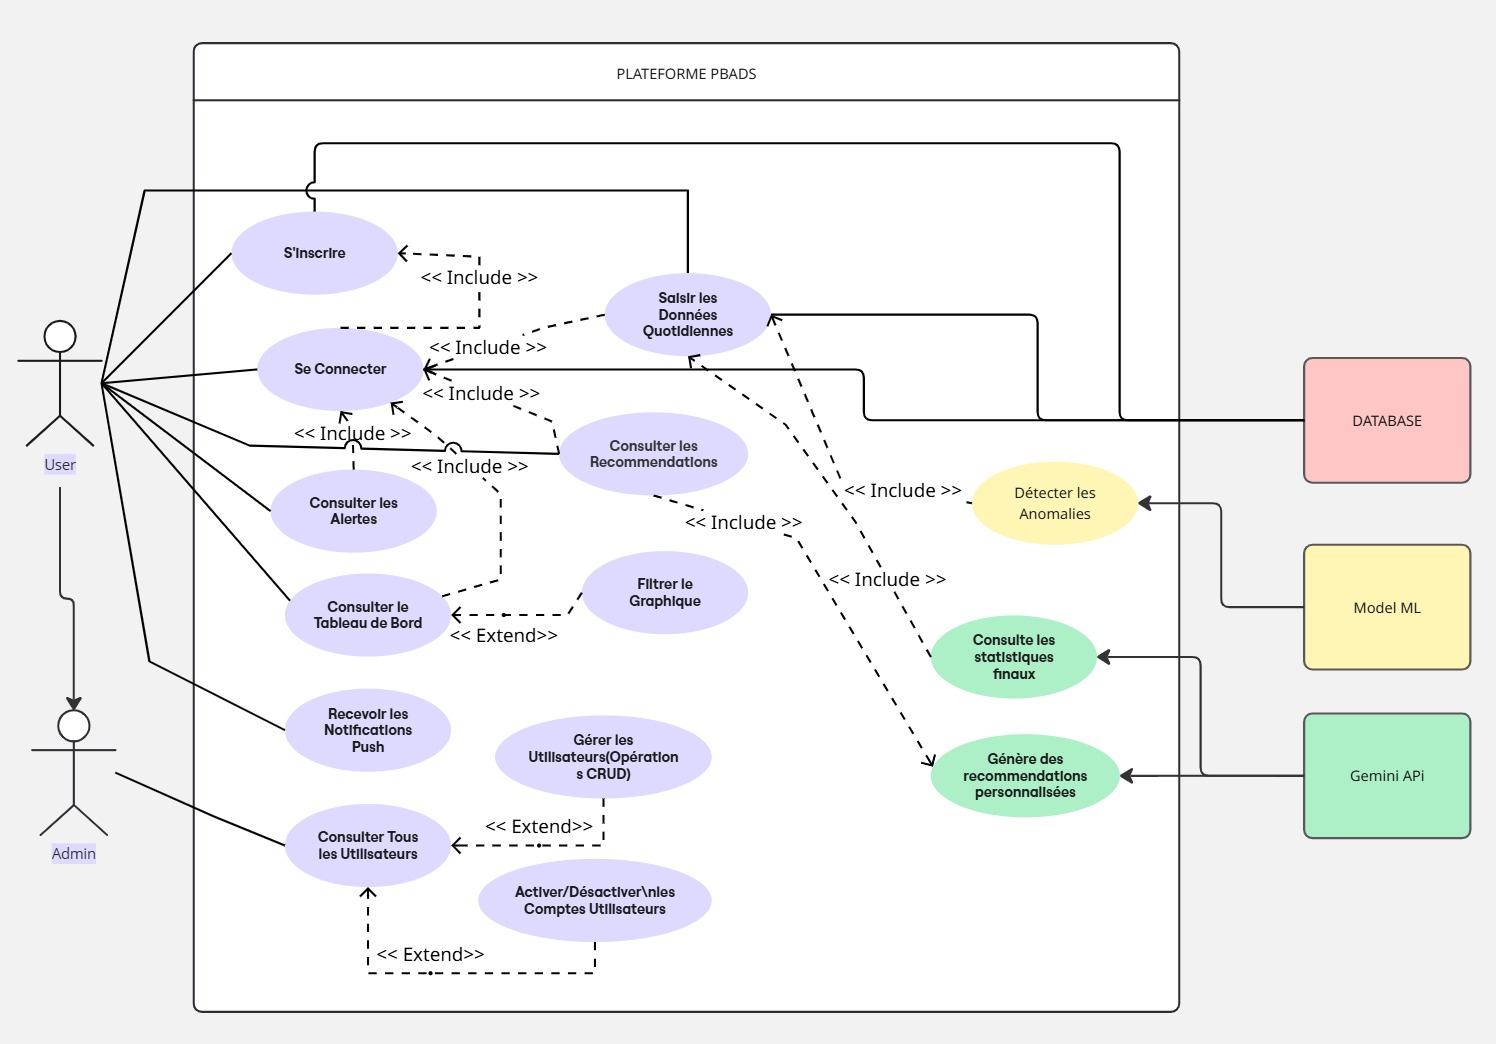
\includegraphics[width=\textwidth]{Figures/pbadsdiags/pbadsusecase.jpg}
    \caption{Diagramme de cas d'utilisation du système PBADS}
    \label{fig:usecase_diagram}
\end{figure}

\textbf{Description du diagramme de cas d'utilisation :}

Le diagramme illustre trois acteurs principaux : \textbf{Utilisateur}, \textbf{Administrateur} (qui hérite de toutes les fonctionnalités utilisateur), et \textbf{Modèle ML}. Les cas d'utilisation sont organisés en trois groupes fonctionnels :

\begin{itemize}
    \item \textbf{Fonctionnalités Utilisateur :} Connexion, inscription, consultation du tableau de bord, saisie des données quotidiennes, consultation des alertes, consultation des recommandations, réception des notifications push, filtrage des graphiques.
    \item \textbf{Fonctionnalités Administrateur :} Gestion des utilisateurs (CRUD), activation/désactivation des comptes, consultation de tous les utilisateurs.
    \item \textbf{Fonctionnalités Modèle ML :} Entraînement, chargement, inférence, détection d'anomalies, stockage, versioning, évaluation.
\end{itemize}

Les relations entre cas d'utilisation incluent des dépendances \texttt{<<include>>} (par exemple, la saisie de données inclut la détection d'anomalies) et des extensions \texttt{<<extend>>} (par exemple, la consultation du tableau de bord peut étendre le filtrage des graphiques).

\subsection{Diagramme de classes}

Le diagramme de classes ci-dessous présente l'architecture complète du système PBADS, illustrant les entités métier principales et leurs relations. Cette modélisation reflète fidèlement l'implémentation technique réalisée avec Spring Boot et JPA.

\begin{figure}[H]
    \centering
    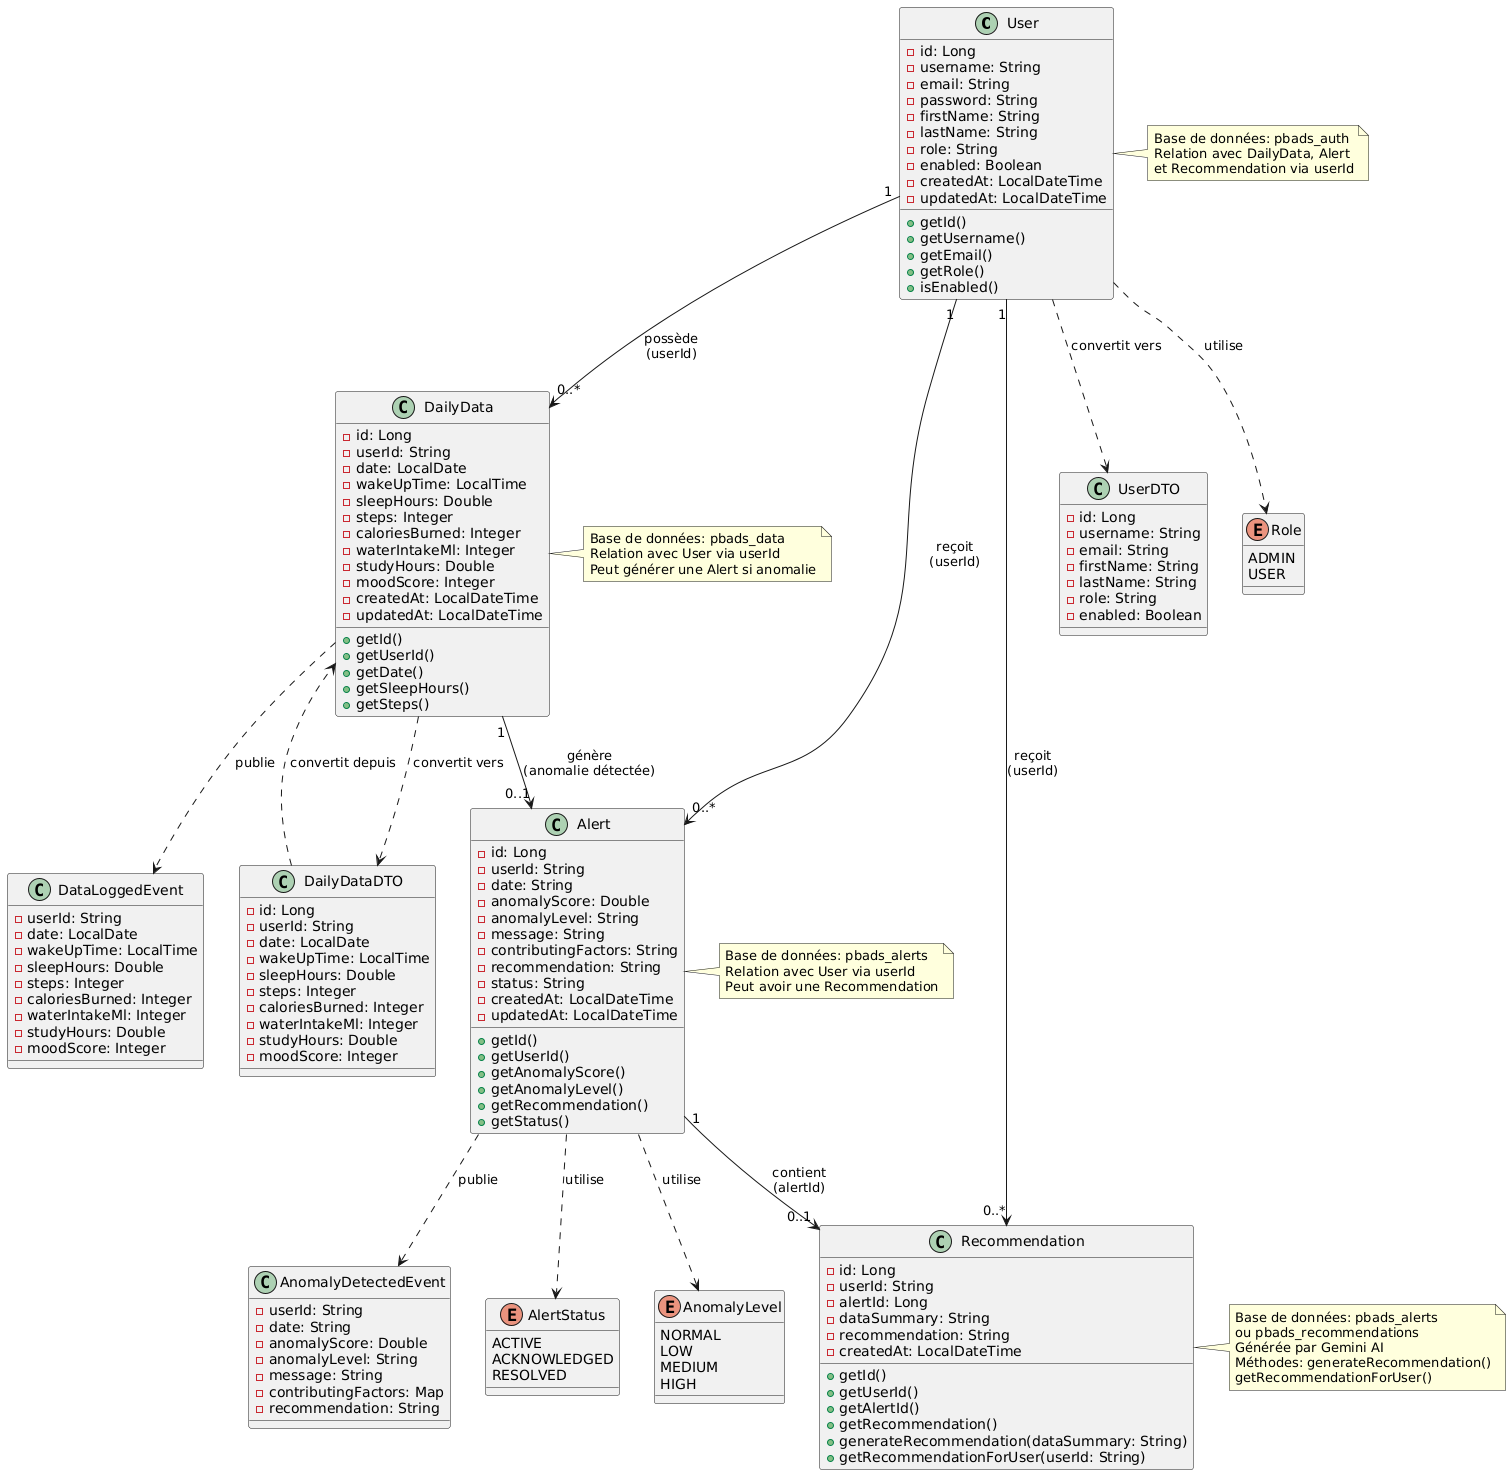
\includegraphics[width=\textwidth]{Figures/pbadsdiags/classdiagram.jpg}
    \caption{Diagramme de classes du système PBADS}
    \label{fig:class_diagram}
\end{figure}

\textbf{Description du diagramme de classes :}

Le modèle de données s'articule autour de trois entités principales : \textbf{User}, \textbf{DailyData}, et \textbf{Alert}. Chaque entité est stockée dans une base de données PostgreSQL distincte selon le principe de l'architecture microservices (une base de données par service).

\textbf{Entités principales :}

\begin{itemize}
    \item \textbf{User :} Gestion des comptes utilisateurs avec authentification JWT, incluant les attributs username, email, password (hashé avec BCrypt), role (ADMIN ou USER), enabled (actif/désactivé), et les timestamps createdAt et updatedAt.
    \item \textbf{DailyData :} Données quotidiennes des utilisateurs avec userId, date, wakeUpTime, sleepHours, steps, caloriesBurned, waterIntakeMl, studyHours, moodScore, et les timestamps createdAt et updatedAt.
    \item \textbf{Alert :} Alertes générées lors de la détection d'anomalies avec userId, date, anomalyScore (0-1), anomalyLevel (NORMAL, LOW, MEDIUM, HIGH), message, contributingFactors (JSON), recommendation (générée par Gemini AI), status (ACTIVE, ACKNOWLEDGED, RESOLVED), et les timestamps createdAt et updatedAt.
    \item \textbf{Recommendation :} Entité représentant les recommandations générées par Google Gemini AI, avec userId, alertId, dataSummary, recommendation, et createdAt. Les méthodes incluent generateRecommendation() et getRecommendationForUser().
\end{itemize}

\textbf{Relations clés :}

Le diagramme illustre les relations cardinales importantes :
\begin{itemize}
    \item Un \textbf{User} (1) peut avoir plusieurs \textbf{DailyData} (0..*) via userId
    \item Un \textbf{User} (1) peut recevoir plusieurs \textbf{Alert} (0..*) via userId
    \item Un \textbf{User} (1) peut recevoir plusieurs \textbf{Recommendation} (0..*) via userId
    \item Une \textbf{DailyData} (1) peut générer une \textbf{Alert} (0..1) si une anomalie est détectée
    \item Une \textbf{Alert} (1) peut avoir une \textbf{Recommendation} (0..1) associée via alertId
\end{itemize}

\textbf{Énumérations :}

Le système utilise plusieurs énumérations pour standardiser les valeurs : \texttt{Role} (ADMIN, USER), \texttt{AlertStatus} (ACTIVE, ACKNOWLEDGED, RESOLVED), et \texttt{AnomalyLevel} (NORMAL, LOW, MEDIUM, HIGH).

Cette architecture garantit l'intégrité des données, la cohérence des relations et la flexibilité nécessaire pour supporter l'évolution future du système.

\subsection{Les diagrammes de séquence}

Cette section présente les flux d'interactions dynamiques entre les différents acteurs du système PBADS. Les diagrammes de séquence suivants décomposent chaque processus en étapes claires, montrant les échanges d'informations entre les acteurs humains et les composants système.

\subsubsection{Scénario : Administrateur interagissant avec la plateforme}

\begin{figure}[H]
    \centering
    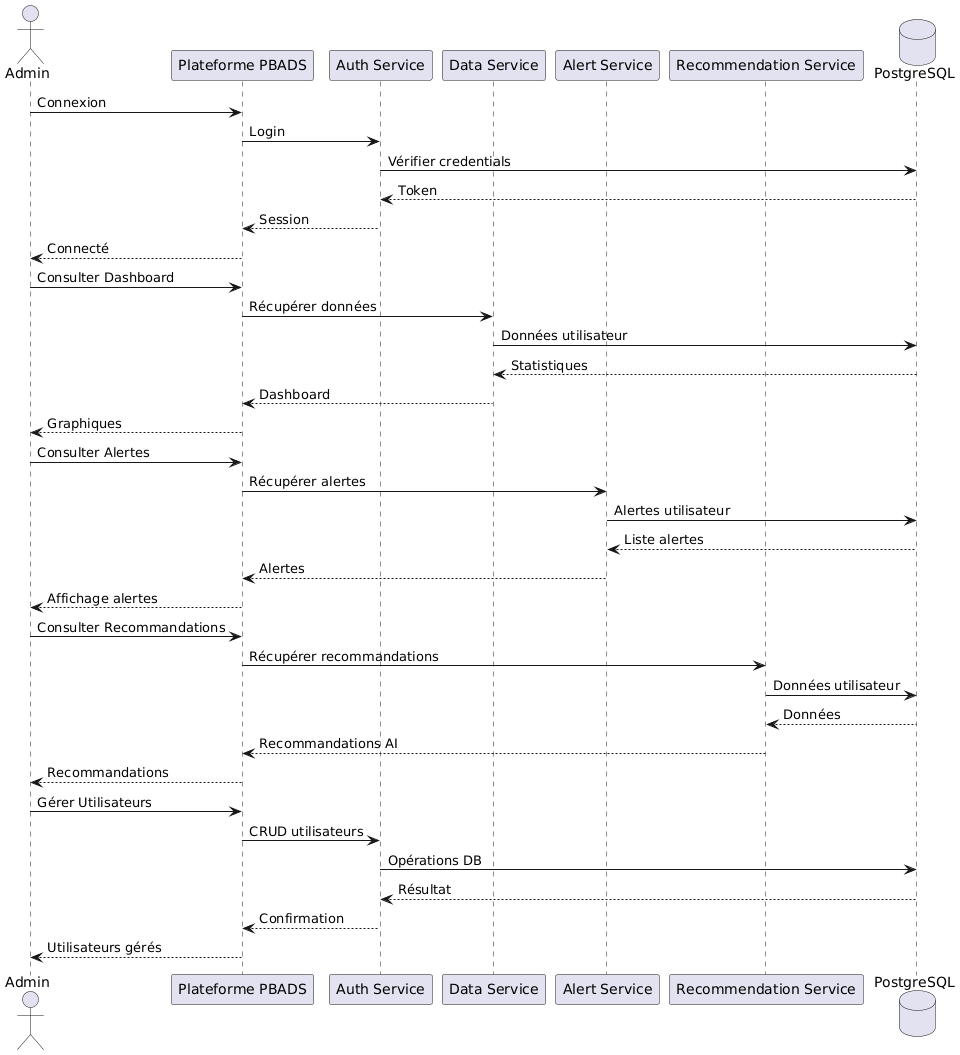
\includegraphics[width=\textwidth]{Figures/pbadsdiags/SequenceAdminPlateform.jpg}
    \caption{Diagramme de séquence - Administrateur interagissant avec la plateforme}
    \label{fig:seq_admin}
\end{figure}

\textbf{Scénario Administrateur (Figure \ref{fig:seq_admin}) :} Ce diagramme illustre les interactions d'un administrateur avec le système PBADS. Le scénario commence par la \textbf{connexion} de l'administrateur via le service d'authentification, qui vérifie les credentials et retourne un token JWT. L'administrateur peut ensuite \textbf{consulter le tableau de bord} en récupérant les données quotidiennes et les recommandations. Il peut également \textbf{consulter les alertes} pour visualiser toutes les alertes générées. Enfin, l'administrateur peut \textbf{gérer les utilisateurs} en effectuant des opérations CRUD (création, lecture, mise à jour, suppression) et activer/désactiver les comptes utilisateurs.

\subsubsection{Scénario : Modèle ML interagissant avec la base de données et la plateforme}

\begin{figure}[H]
    \centering
    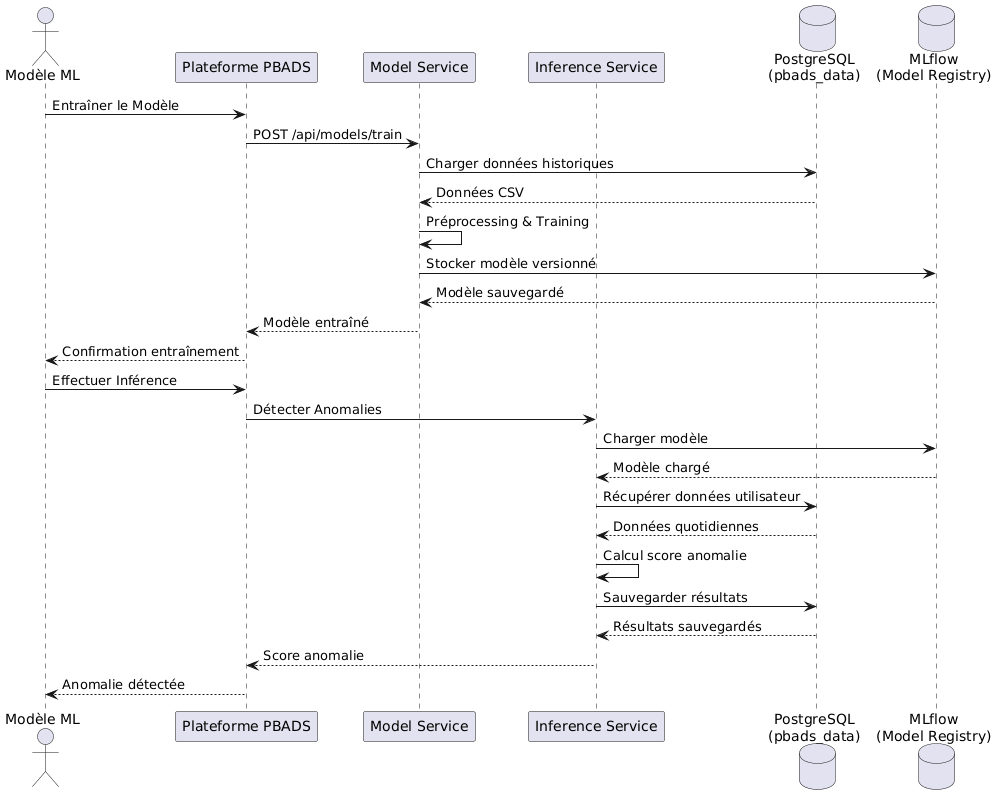
\includegraphics[width=\textwidth]{Figures/pbadsdiags/SequenceModelePlateformeDB.jpg}
    \caption{Diagramme de séquence - Modèle ML interagissant avec la base de données et la plateforme}
    \label{fig:seq_modele}
\end{figure}

\textbf{Scénario Modèle ML (Figure \ref{fig:seq_modele}) :} Ce diagramme détaille les interactions du modèle ML avec la plateforme et les bases de données. Le scénario commence par l'\textbf{entraînement du modèle} où le Model Service charge les données historiques depuis la base de données, effectue le preprocessing et l'entraînement, puis stocke le modèle versionné dans MLflow. Lors de l'\textbf{inférence}, le Inference Service charge le modèle depuis MLflow, récupère les données utilisateur depuis la base de données, calcule le score d'anomalie, et sauvegarde les résultats. Si une anomalie est détectée, une alerte est générée avec les détails de l'anomalie.

\section{Conclusion}

Ce chapitre a présenté la modélisation complète du système PBADS, couvrant l'analyse des besoins, la définition des objectifs, la méthodologie agile adoptée, et la modélisation conceptuelle détaillée avec les diagrammes UML. L'étude des lacunes des solutions existantes a permis d'identifier les besoins critiques en matière de détection automatique d'anomalies, de génération de recommandations personnalisées, et de visualisation interactive des données.

Les diagrammes UML (cas d'utilisation, classes et séquences) fournissent une vision claire de l'architecture et des interactions du système. Cette modélisation constitue la base solide pour l'implémentation technique qui sera détaillée dans le chapitre suivant.


% --- Chapter 3 ---
\chaptertitlepage{Interfaces et Réalisation de l'application}
% Résumé pour la page de titre du chapitre 3
\begin{flushright}
\begin{minipage}{0.6\textwidth}
Ce chapitre présente les technologies utilisées, l'architecture microservices, et les interfaces développées pour le système PBADS. Il détaille l'implémentation technique des microservices, les choix technologiques (Spring Boot, Kafka, PostgreSQL, scikit-learn, Google Gemini AI), et les interfaces utilisateur avec thème sombre moderne. Cette approche modulaire facilite la maintenance, l'évolution et la scalabilité de la solution.
\end{minipage}
\end{flushright}
\clearpage
Ce chapitre présente les technologies utilisées, l'architecture technique, et les interfaces développées pour le système PBADS.

\section{Technologies et Architecture}

\subsection{Architecture microservices}

Notre système suit une architecture microservices moderne, séparant clairement les responsabilités entre les différents services pour garantir la scalabilité, la maintenabilité et la tolérance aux pannes.

\textbf{Composants de l'architecture :}

\begin{itemize}
    \item \textbf{Frontend (Thymeleaf) :} Interface utilisateur développée avec Thymeleaf et Chart.js
    \item \textbf{Backend (Spring Boot) :} APIs REST développées avec Spring Boot
    \item \textbf{Bases de données (PostgreSQL) :} Bases de données relationnelles avec JPA/Hibernate
    \item \textbf{Sécurité :} Authentification JWT et contrôle d'accès basé sur les rôles
    \item \textbf{Communication :} Kafka pour la messagerie asynchrone et HTTP/REST pour les appels synchrones
    \item \textbf{Machine Learning :} Python (scikit-learn) pour l'entraînement et l'inférence des modèles
    \item \textbf{IA :} Google Gemini AI pour la génération de recommandations personnalisées
\end{itemize}

\subsection{Technologies Frontend}

\subsubsection{Thymeleaf}

Thymeleaf constitue le moteur de template côté serveur pour notre interface utilisateur, offrant une intégration native avec Spring MVC.

\textbf{Composants principaux :}
\begin{itemize}
    \item \textbf{Templates :} Pages HTML avec syntaxe Thymeleaf pour le rendu dynamique
    \item \textbf{Fragments :} Composants réutilisables (navbar, footer)
    \item \textbf{Expressions :} Accès aux données du modèle et aux variables de session
    \item \textbf{Sécurité :} Intégration avec Spring Security pour la protection des routes
\end{itemize}

\subsubsection{Chart.js}

Chart.js fournit une bibliothèque de graphiques JavaScript pour la visualisation interactive des données comportementales.

\textbf{Composants utilisés :}
\begin{itemize}
    \item \textbf{Graphiques linéaires :} Visualisation des tendances comportementales dans le temps
    \item \textbf{Filtres temporels :} Filtrage par semaine, mois, année, ou toutes les données
    \item \textbf{Animations :} Transitions fluides lors du changement de filtres
    \item \textbf{Thème sombre :} Interface adaptée avec palette de couleurs personnalisée
\end{itemize}

\subsection{Technologies Backend}

\subsubsection{Spring Boot Framework}

Spring Boot constitue la base de nos APIs REST, offrant une configuration simplifiée et des fonctionnalités enterprise robustes.

\textbf{Modules Spring utilisés :}
\begin{itemize}
    \item \textbf{Spring Web :} Développement d'API REST avec annotations
    \item \textbf{Spring Security :} Gestion de la sécurité et de l'authentification
    \item \textbf{Spring Data JPA :} Abstraction de la couche de données
    \item \textbf{Spring Cloud Gateway :} Point d'entrée unique pour toutes les requêtes
    \item \textbf{Spring Cloud Eureka :} Découverte de services
    \item \textbf{Spring Cloud Config :} Configuration centralisée
    \item \textbf{Spring Cloud OpenFeign :} Client HTTP déclaratif pour la communication entre services
\end{itemize}

\subsubsection{Kafka}

Apache Kafka est utilisé comme broker de messagerie pour la communication asynchrone entre services.

\textbf{Topics utilisés :}
\begin{itemize}
    \item \texttt{data.logged.events} : Événements de données quotidiennes enregistrées
    \item \texttt{anomaly.detected.events} : Événements d'anomalies détectées
\end{itemize}

\subsubsection{PostgreSQL Database}

PostgreSQL a été choisi comme base de données relationnelle pour sa robustesse et ses performances.

\textbf{Bases de données :}
\begin{itemize}
    \item \texttt{pbads\_auth} : Données d'authentification et utilisateurs
    \item \texttt{pbads\_data} : Données quotidiennes des utilisateurs
    \item \texttt{pbads\_alerts} : Alertes générées
\end{itemize}

\subsection{Machine Learning}

\subsubsection{scikit-learn}

scikit-learn est utilisé pour l'entraînement et l'inférence des modèles de détection d'anomalies.

\textbf{Algorithmes utilisés :}
\begin{itemize}
    \item \textbf{Isolation Forest :} Algorithme principal pour la détection d'anomalies
    \item \textbf{One-Class SVM :} Algorithme alternatif avec noyau RBF
\end{itemize}

\subsubsection{MLflow}

MLflow est utilisé pour le suivi des expériences ML et le versioning des modèles.

\section{Interfaces Utilisateur}

Cette section présente les interfaces développées pour les utilisateurs et les administrateurs du système PBADS.

\subsection{Vue Utilisateur}

\subsubsection{Page d'inscription}

\begin{figure}[H]
    \centering
    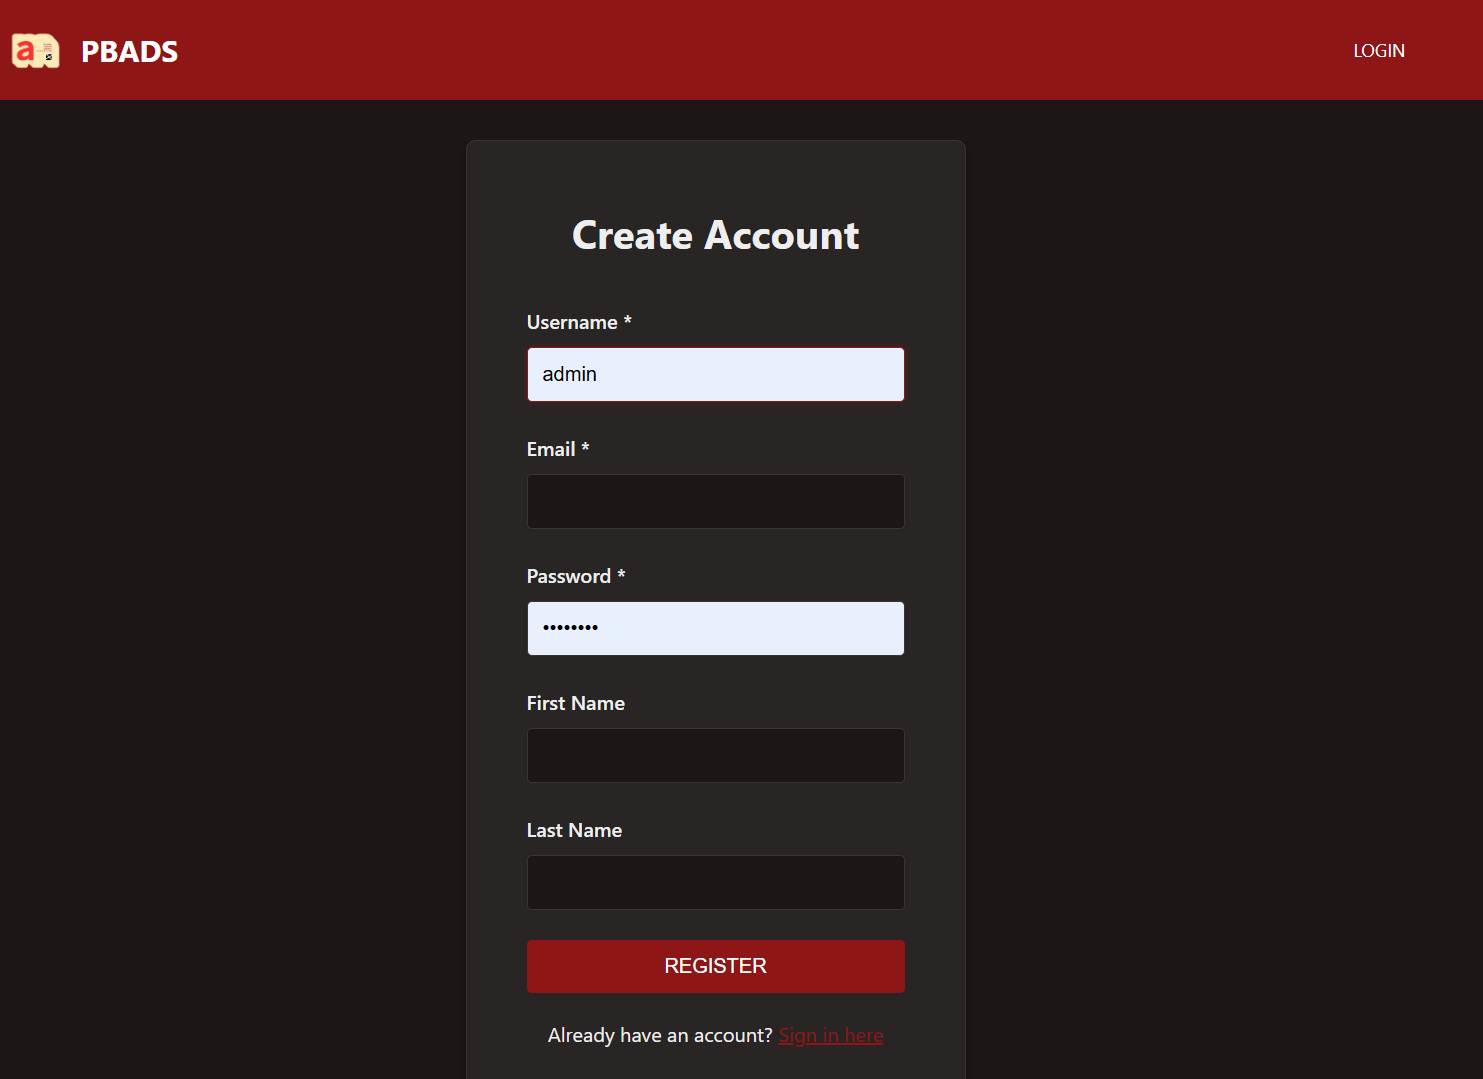
\includegraphics[width=\textwidth]{Figures/pbadsuser/userregisterpage.png}
    \caption{Page d'inscription - Création de compte utilisateur}
    \label{fig:user-register}
\end{figure}

Cette interface permet aux nouveaux utilisateurs de créer un compte dans le système PBADS. Le formulaire collecte les informations essentielles : nom d'utilisateur, email, mot de passe, et prénom/nom. La page utilise un thème sombre moderne avec une navigation simplifiée (seul le lien "LOGIN" est visible pour les utilisateurs non authentifiés).

\subsubsection{Page de connexion}

\begin{figure}[H]
    \centering
    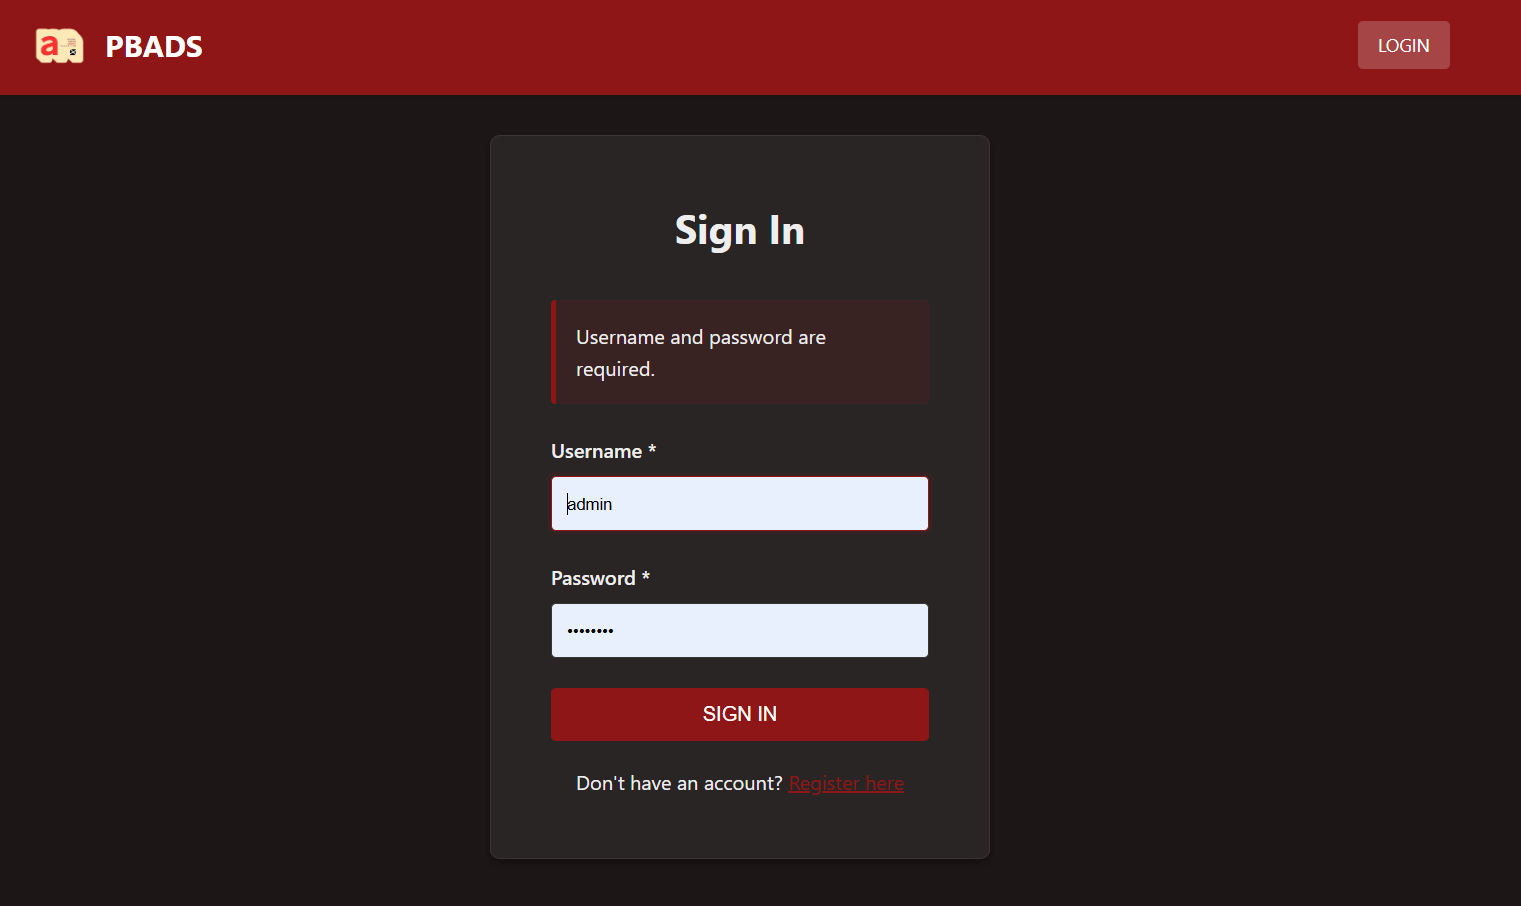
\includegraphics[width=\textwidth]{Figures/pbadsuser/usersigninpage.png}
    \caption{Page de connexion - Authentification utilisateur}
    \label{fig:user-signin}
\end{figure}

Cette interface permet aux utilisateurs de se connecter au système avec leurs identifiants (nom d'utilisateur et mot de passe). La page suit le même thème sombre cohérent avec le reste de l'application et offre un accès rapide à la page d'inscription pour les nouveaux utilisateurs.

\subsubsection{Tableau de bord - Graphiques}

\begin{figure}[H]
    \centering
    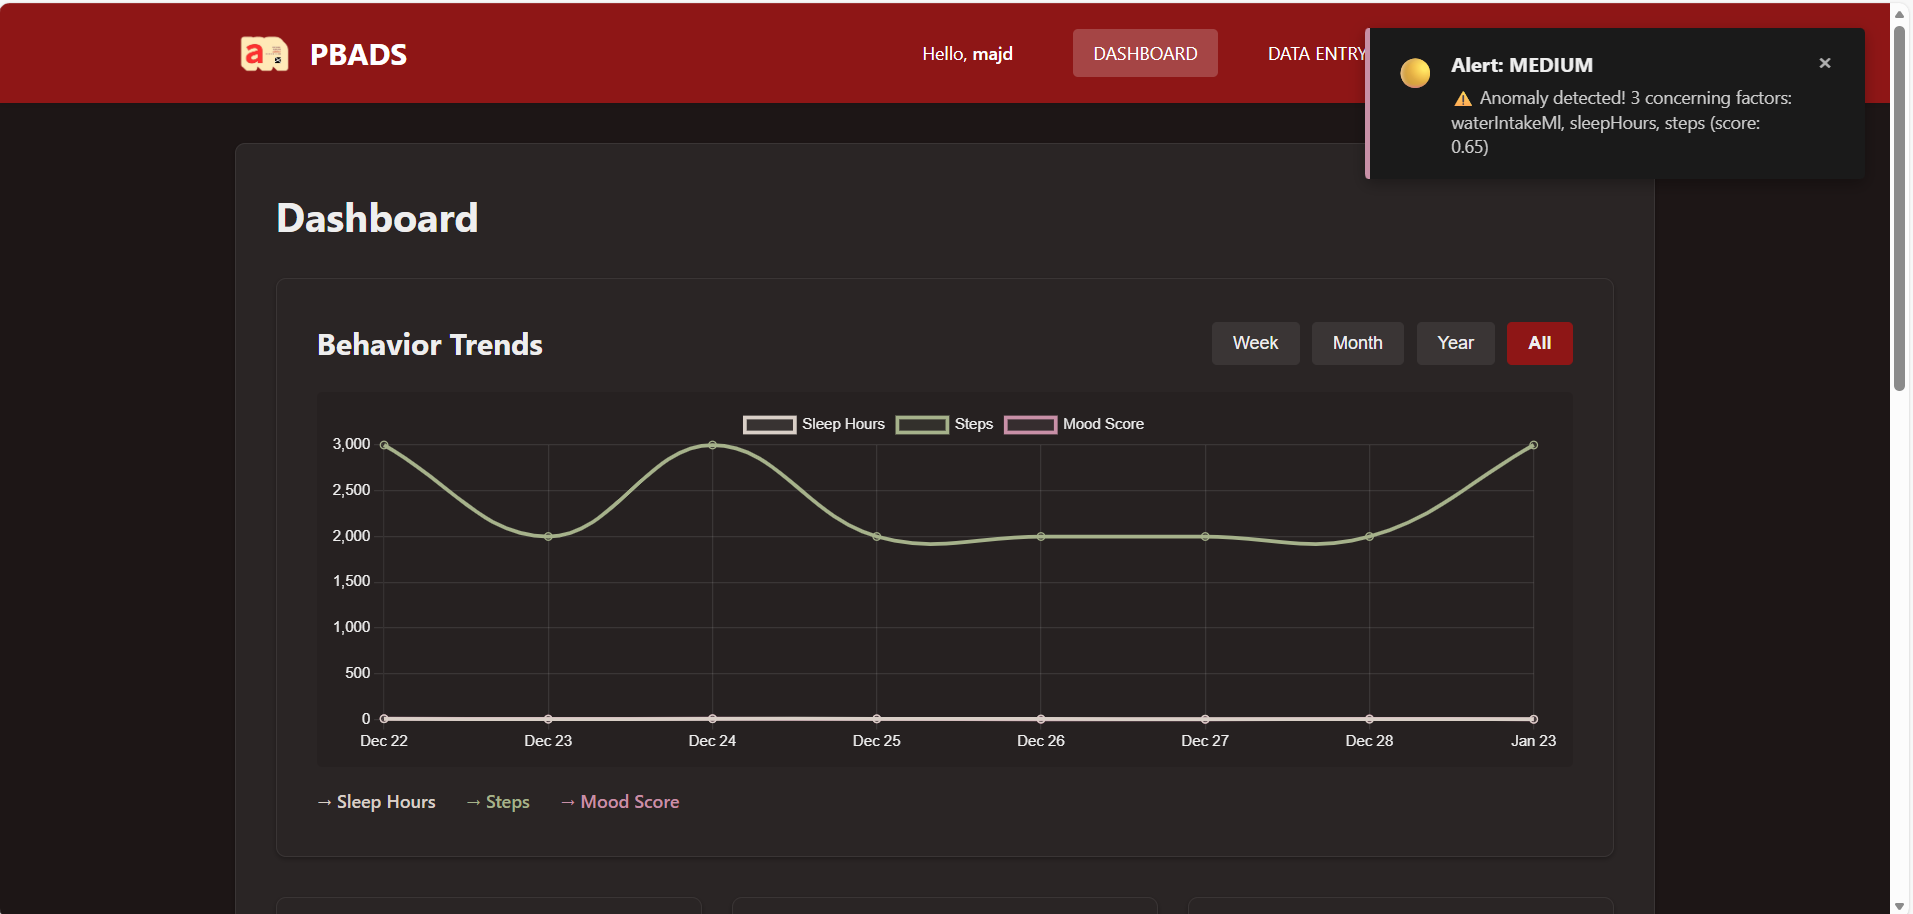
\includegraphics[width=\textwidth]{Figures/pbadsuser/userdashboardgraph.png}
    \caption{Tableau de bord - Visualisation des tendances comportementales}
    \label{fig:user-dashboard-graph}
\end{figure}

Cette interface constitue le cœur du système PBADS, présentant une visualisation interactive des données comportementales de l'utilisateur. Le tableau de bord inclut :

\begin{itemize}
    \item \textbf{Graphique des tendances comportementales :} Visualisation des données quotidiennes avec Chart.js
    \item \textbf{Filtres temporels :} Boutons pour filtrer par semaine, mois, année, ou toutes les données
    \item \textbf{Statistiques résumées :} Vue d'ensemble des métriques clés (sommeil moyen, steps moyens, etc.)
    \item \textbf{Thème sombre :} Interface moderne avec palette de couleurs personnalisée (\#1a1a1a, \#2d2d2d, \#8E1616)
\end{itemize}

\subsubsection{Tableau de bord - Alertes et Recommandations}

\begin{figure}[H]
    \centering
    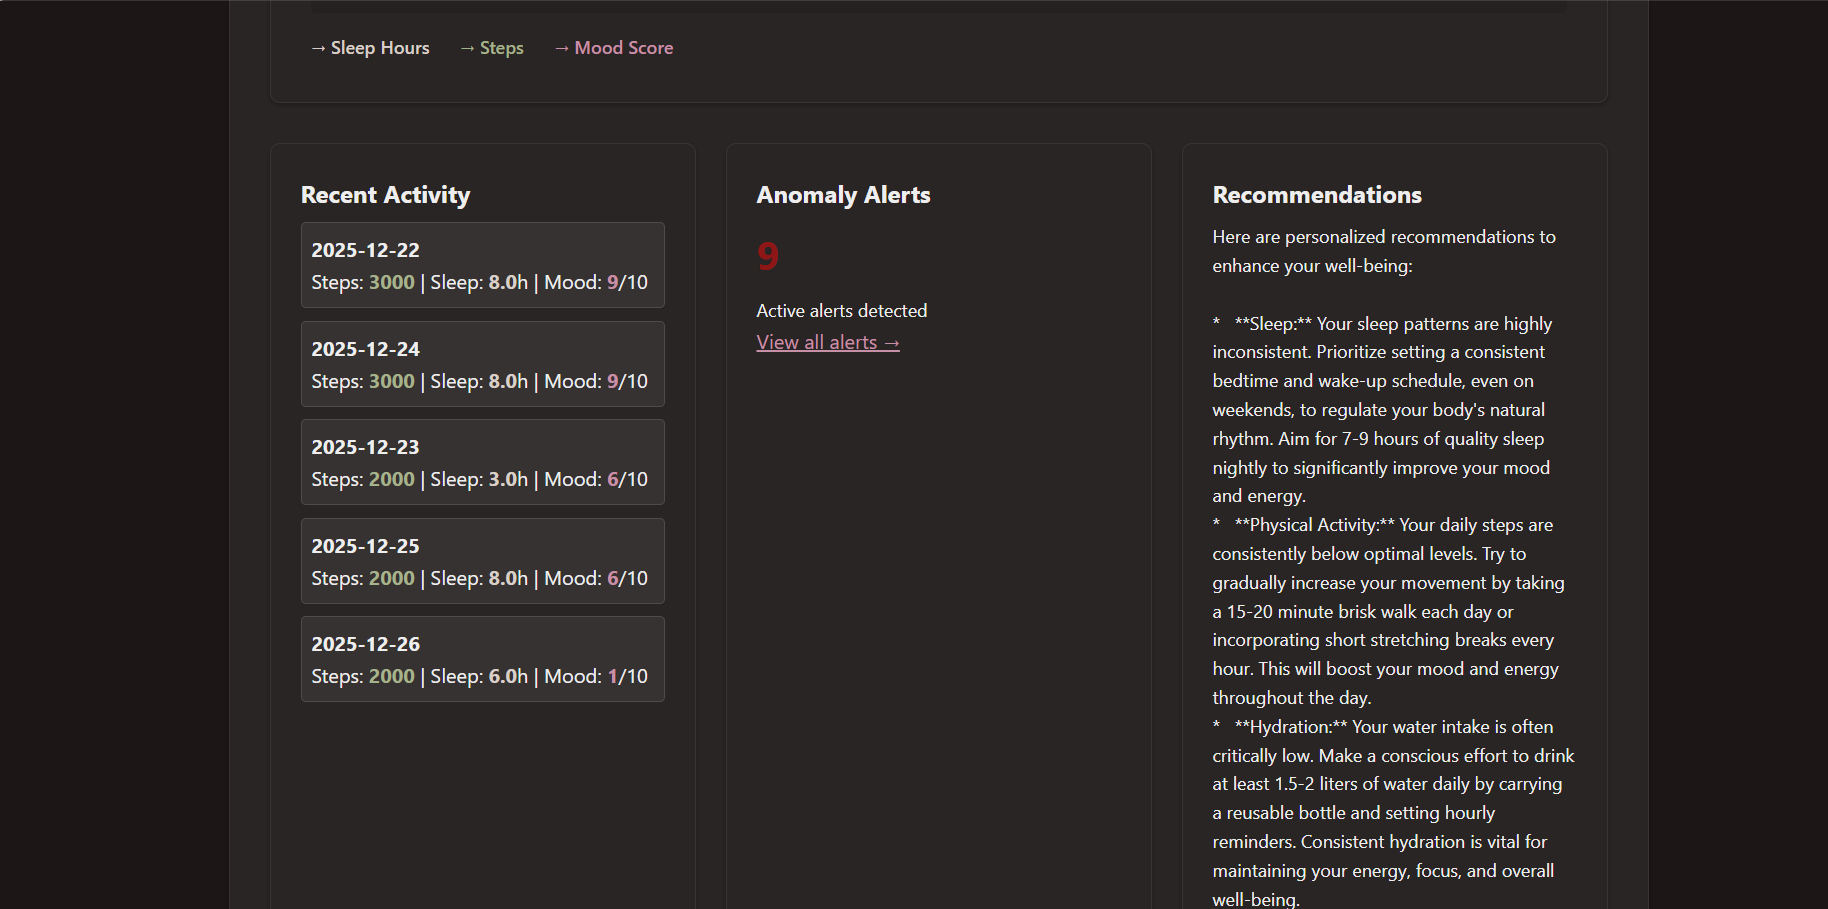
\includegraphics[width=\textwidth]{Figures/pbadsuser/userdashboardalertsandrecommandation.png}
    \caption{Tableau de bord - Alertes et recommandations IA}
    \label{fig:user-dashboard-alerts}
\end{figure}

Cette section du tableau de bord présente les alertes générées et les recommandations personnalisées. L'interface affiche :

\begin{itemize}
    \item \textbf{Alertes récentes :} Liste des alertes avec niveaux de sévérité (HIGH, MEDIUM, LOW)
    \item \textbf{Recommandations IA :} Suggestions personnalisées générées par Google Gemini AI
    \item \textbf{Badges de statut :} Indicateurs visuels pour les niveaux d'alerte
    \item \textbf{Design cohérent :} Intégration harmonieuse avec le thème sombre du tableau de bord
\end{itemize}

\subsubsection{Saisie de données quotidiennes}

\begin{figure}[H]
    \centering
    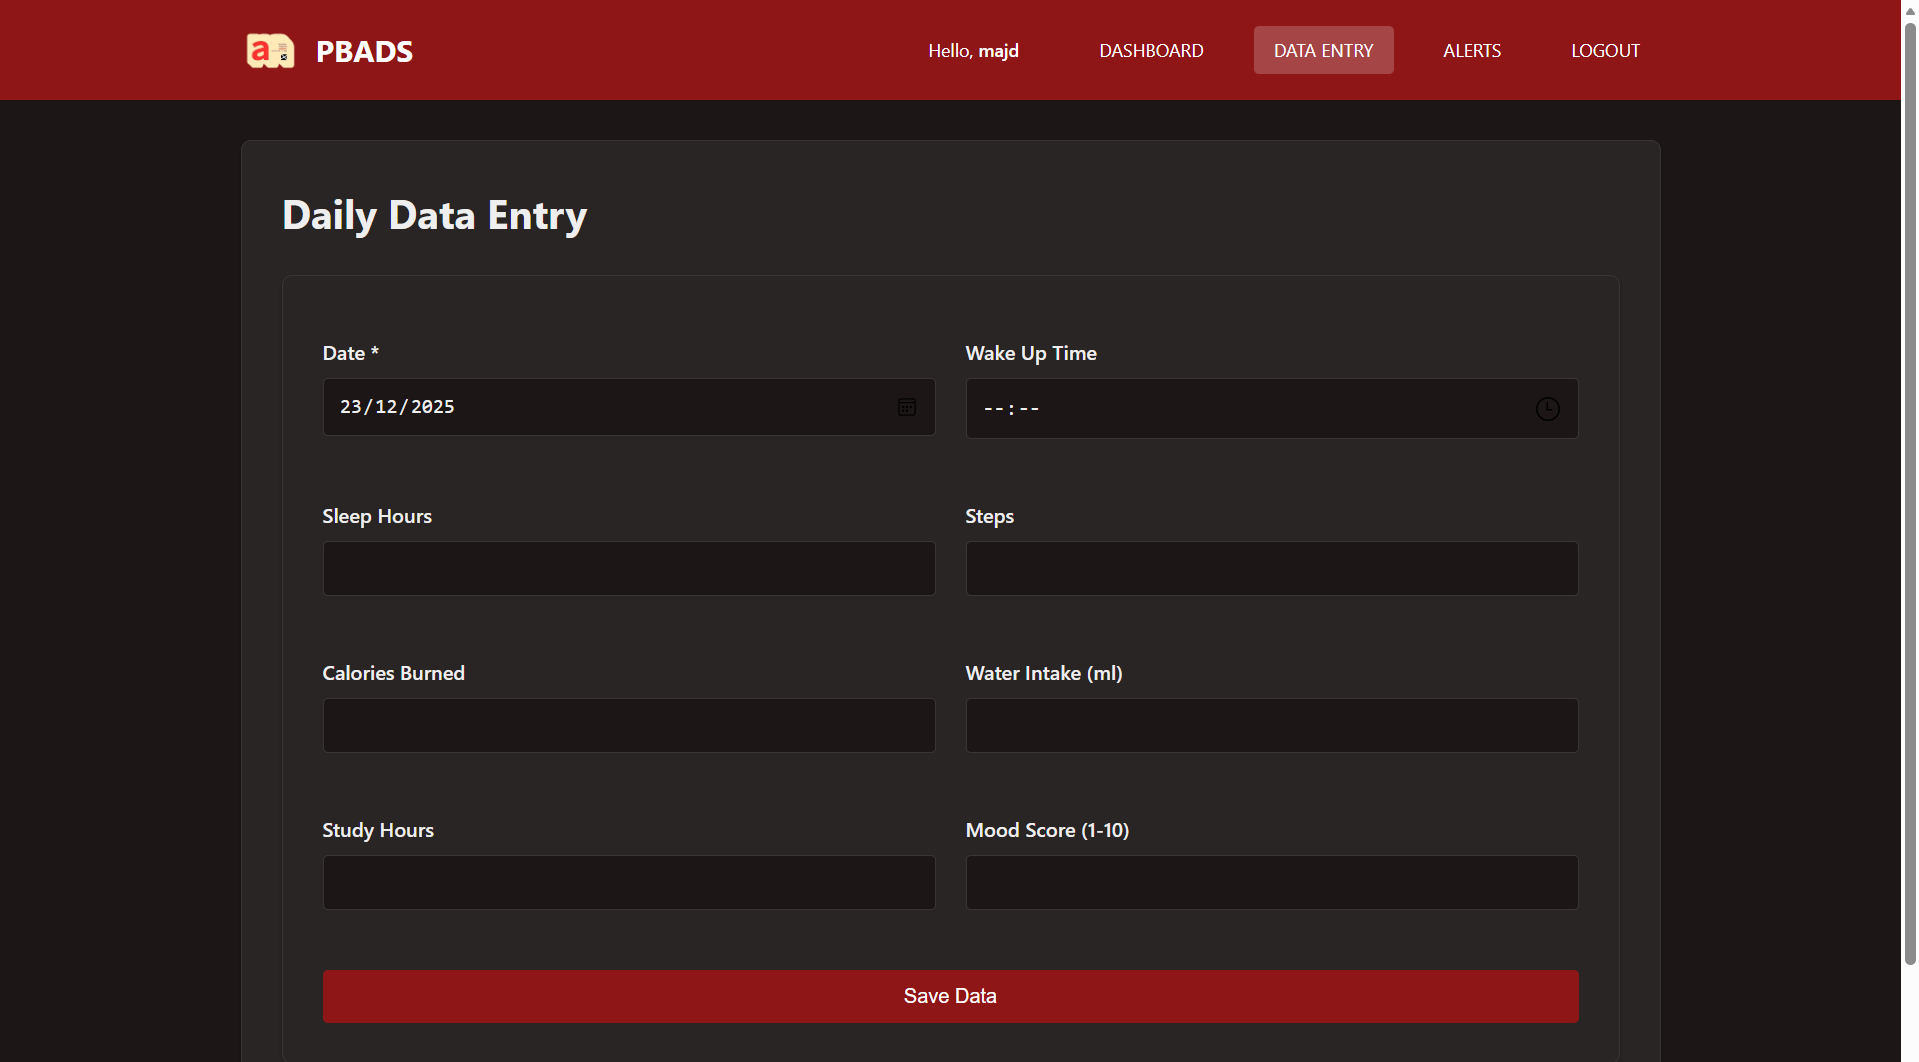
\includegraphics[width=\textwidth]{Figures/pbadsuser/userdataentry.png}
    \caption{Formulaire de saisie des données quotidiennes}
    \label{fig:user-data-entry}
\end{figure}

Cette interface permet aux utilisateurs de saisir leurs données quotidiennes de manière structurée. Le formulaire inclut :

\begin{itemize}
    \item \textbf{Date :} Sélection de la date pour laquelle les données sont enregistrées
    \item \textbf{Heure de réveil :} Champ pour l'heure de réveil
    \item \textbf{Heures de sommeil :} Nombre d'heures de sommeil
    \item \textbf{Steps :} Nombre de pas effectués dans la journée
    \item \textbf{Calories brûlées :} Nombre de calories brûlées
    \item \textbf{Consommation d'eau :} Quantité d'eau consommée en millilitres
    \item \textbf{Heures d'étude :} Temps consacré à l'étude
    \item \textbf{Score d'humeur :} Évaluation de l'humeur sur une échelle de 1 à 10
\end{itemize}

Le formulaire utilise une validation côté client et serveur pour garantir l'intégrité des données.

\subsubsection{Notification push d'alerte}

\begin{figure}[H]
    \centering
    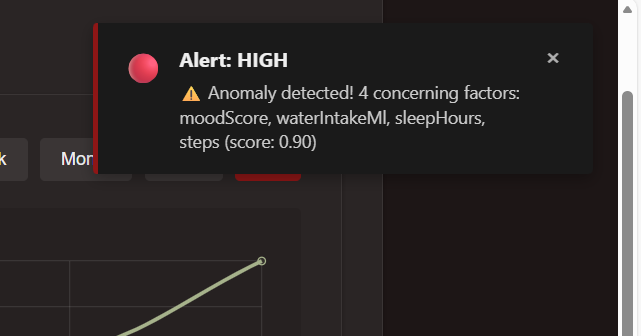
\includegraphics[width=\textwidth]{Figures/pbadsuser/userpushalert.png}
    \caption{Notification push - Alerte d'anomalie détectée}
    \label{fig:user-push-alert}
\end{figure}

Cette interface illustre le système de notifications push (toast) qui alerte les utilisateurs en temps réel lorsqu'une nouvelle anomalie est détectée. Les caractéristiques incluent :

\begin{itemize}
    \item \textbf{Notification éphémère :} Affichage temporaire en haut à droite de l'écran
    \item \textbf{Niveaux de sévérité :} Couleurs différentes selon le niveau (HIGH, MEDIUM, LOW)
    \item \textbf{Message informatif :} Description de l'anomalie détectée
    \item \textbf{Bouton de fermeture :} Possibilité de fermer manuellement la notification
    \item \textbf{Animation :} Transitions fluides pour l'apparition et la disparition
\end{itemize}

Le système poll le service d'alertes toutes les 5 secondes pour détecter les nouvelles alertes et afficher les notifications automatiquement.

\subsubsection{Page des alertes}

\begin{figure}[H]
    \centering
    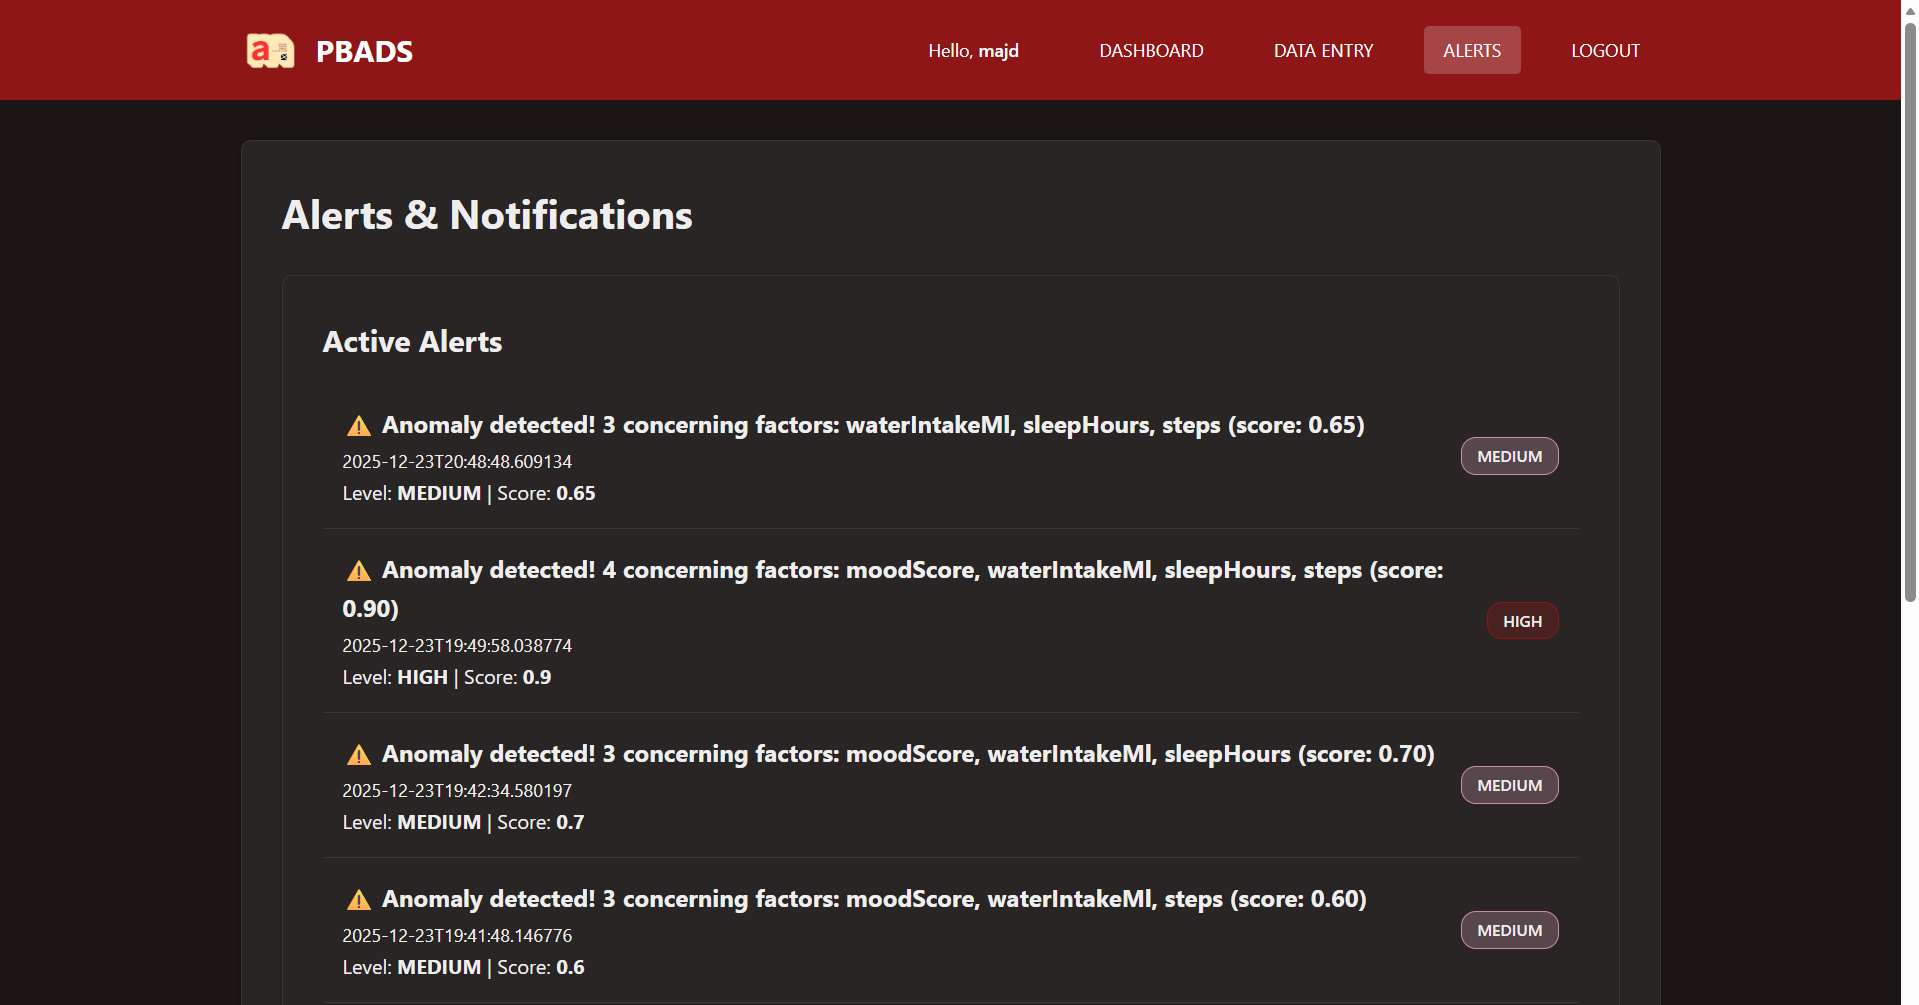
\includegraphics[width=\textwidth]{Figures/pbadsuser/useralertpage.png}
    \caption{Page de consultation des alertes}
    \label{fig:user-alert-page}
\end{figure}

Cette interface permet aux utilisateurs de consulter toutes leurs alertes de manière organisée. La page affiche :

\begin{itemize}
    \item \textbf{Liste complète des alertes :} Toutes les alertes générées pour l'utilisateur
    \item \textbf{Informations détaillées :} Date, score d'anomalie, niveau, message
    \item \textbf{Statut des alertes :} Indicateurs visuels pour ACTIVE, ACKNOWLEDGED, RESOLVED
    \item \textbf{Organisation temporelle :} Alertes triées par date (plus récentes en premier)
    \item \textbf{Design cohérent :} Thème sombre avec badges colorés pour les niveaux de sévérité
\end{itemize}

\subsection{Vue Administrateur}

\subsubsection{Gestion des utilisateurs}

\begin{figure}[H]
    \centering
    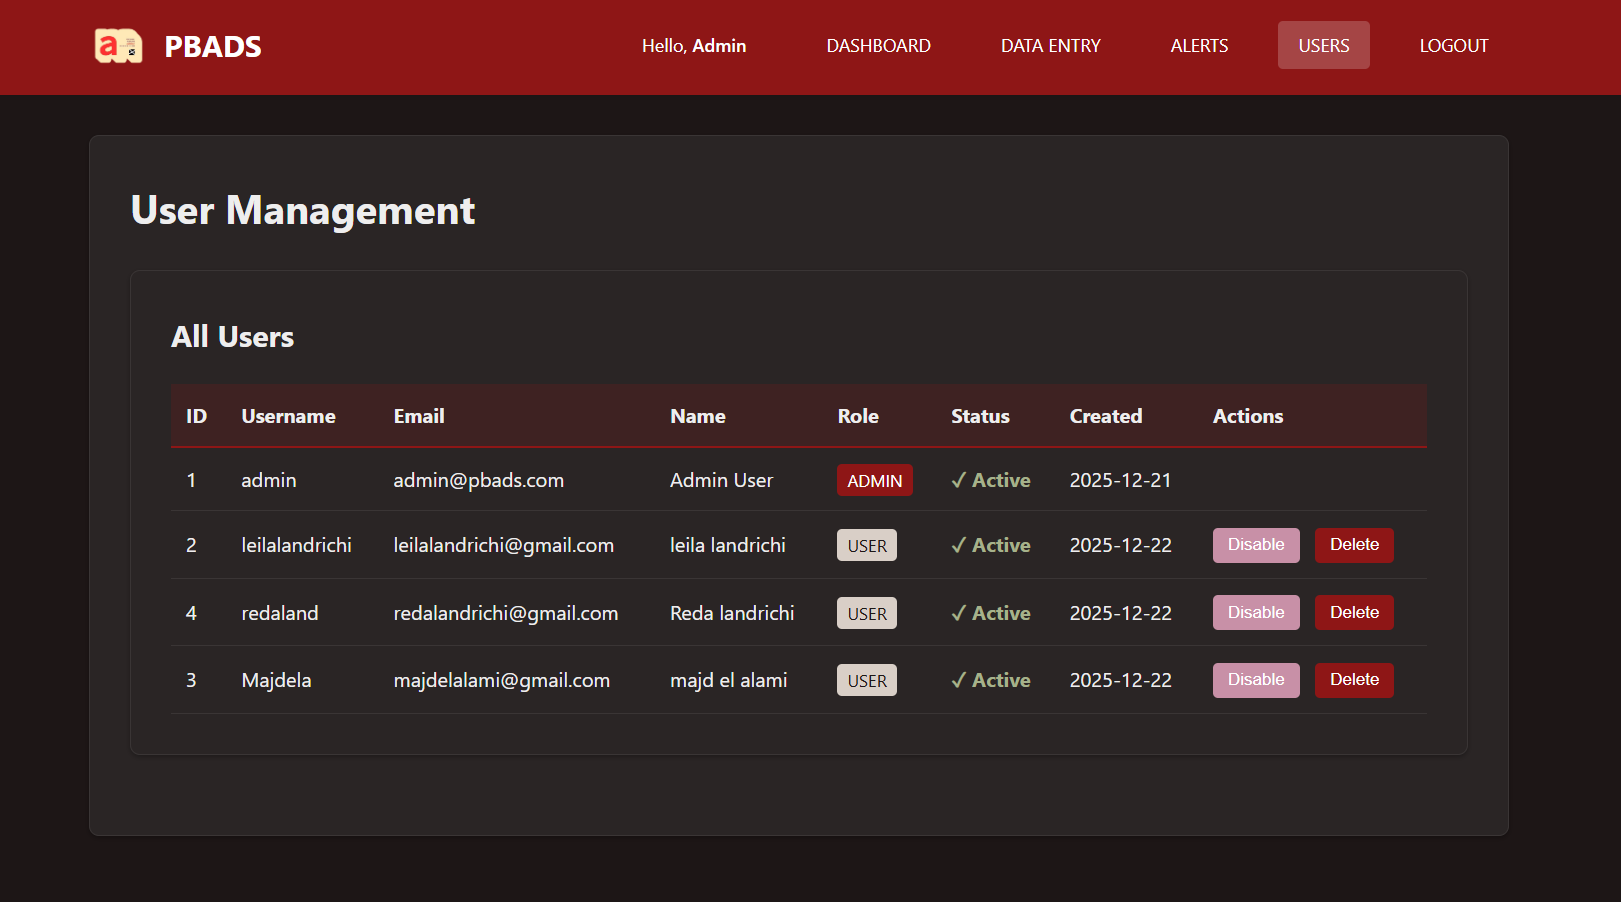
\includegraphics[width=\textwidth]{Figures/pbadsadmin/usermanagement.png}
    \caption{Interface de gestion des utilisateurs (Administrateur)}
    \label{fig:admin-user-management}
\end{figure}

Cette interface permet à l'administrateur de gérer tous les utilisateurs du système. Les fonctionnalités incluent :

\begin{itemize}
    \item \textbf{Liste complète des utilisateurs :} Affichage de tous les comptes utilisateurs
    \item \textbf{Opérations CRUD :} Création, lecture, mise à jour et suppression d'utilisateurs
    \item \textbf{Gestion des rôles :} Attribution des rôles ADMIN ou USER
    \item \textbf{Activation/Désactivation :} Contrôle de l'état actif/inactif des comptes
    \item \textbf{Informations détaillées :} Affichage des données utilisateur (nom d'utilisateur, email, rôle, statut)
    \item \textbf{Interface moderne :} Tableau responsive avec actions rapides
\end{itemize}

L'administrateur hérite de toutes les fonctionnalités utilisateur (tableau de bord, saisie de données, consultation des alertes) en plus de ces fonctionnalités de gestion.

\section{Conclusion}

Ce chapitre a présenté l'implémentation technique complète du système PBADS, couvrant l'architecture microservices, les technologies utilisées, et les interfaces développées pour les utilisateurs et les administrateurs.

L'architecture technique choisie, basée sur Spring Boot et Thymeleaf, offre une base solide et moderne pour le développement d'APIs REST robustes et performantes. L'utilisation de PostgreSQL avec JPA/Hibernate garantit une gestion efficace des données, tandis que l'intégration Kafka assure la communication asynchrone entre services. L'authentification JWT et le contrôle d'accès basé sur les rôles assurent une sécurité renforcée.

Les interfaces développées privilégient l'expérience utilisateur avec un thème sombre moderne, des graphiques interactifs avec Chart.js, et un système de notifications push en temps réel. Chaque rôle dispose d'interfaces adaptées à ses besoins spécifiques, facilitant ainsi l'adoption et l'efficacité du système.

Cette approche modulaire facilite la maintenance, l'évolution et l'adaptation de la solution aux besoins changeants, tout en garantissant une implémentation cohérente et robuste du système PBADS.

% --- FIN DU BLOC AJOUTÉ POUR LE CHAPITRE 4 ---
% Conclusion
\chaptertitlepagenonum{Conclusion générale}
\clearpage
La réalisation du \textbf{Personal Behavior Anomaly Detection System (PBADS)} a constitué une étape majeure de notre parcours académique.

Ce projet nous a confrontés à un défi essentiel : concevoir une solution numérique capable d'analyser les comportements quotidiens des utilisateurs, de détecter automatiquement les anomalies à l'aide d'algorithmes d'apprentissage automatique, et de générer des recommandations personnalisées pour améliorer la qualité de vie.

Nous avons conçu, développé et mis en service un système fonctionnel basé sur une architecture microservices qui automatise la détection d'anomalies comportementales, génère des alertes intelligentes avec niveaux de sévérité, et fournit des recommandations personnalisées via l'intégration avec Google Gemini AI. L'application permet désormais une analyse en temps réel des habitudes de vie, un suivi précis des tendances comportementales, ainsi qu'une visualisation interactive des données via un tableau de bord moderne avec filtres temporels.

Tout au long de ce projet, nous avons su relever plusieurs défis techniques et organisationnels, notamment la modélisation des besoins utilisateurs avec les diagrammes UML, la conception d'une architecture microservices robuste avec Spring Boot, l'intégration de mécanismes d'authentification JWT et de contrôle d'accès basé sur les rôles, l'implémentation de la communication asynchrone avec Kafka et synchrone avec HTTP/REST, l'intégration d'algorithmes de machine learning (Isolation Forest, One-Class SVM) pour la détection d'anomalies, l'intégration avec Google Gemini AI pour la génération de recommandations, et l'optimisation de l'ergonomie des interfaces avec un thème sombre moderne et des graphiques interactifs.

Le respect des contraintes de délai, la rigueur dans la planification agile par itérations, et l'esprit collaboratif au sein de notre équipe ont été des facteurs clés dans l'atteinte de nos objectifs.

Cette expérience nous a permis de renforcer nos compétences en développement fullstack, en architecture microservices, en machine learning, ainsi qu'en intégration d'APIs d'intelligence artificielle.

Elle nous a aussi sensibilisés à l'importance d'une documentation claire, de cycles de test rigoureux, de la modélisation UML pour la compréhension des besoins, et de la prise en compte continue des retours utilisateurs pour garantir la qualité et l'évolutivité du produit.

À l'avenir, nous prévoyons d'enrichir le système avec des fonctionnalités supplémentaires telles qu'une analyse prédictive plus avancée, une intégration avec des dispositifs IoT (montres intelligentes, capteurs), une personnalisation accrue des recommandations basée sur l'historique utilisateur, ou encore une application mobile native pour un suivi encore plus pratique.

En résumé, cette réalisation a été une aventure formatrice et stimulante.

Nous sommes fiers du système que nous avons mis en place et restons motivés à poursuivre son amélioration pour répondre toujours mieux aux besoins d'une détection d'anomalies comportementales moderne, intelligente et accessible.

% --- BIBLIOGRAPHIE ---
\clearpage
\nocite{*}
\printbibliography[heading=bibintoc, title={Bibliographie}]
%======================================================================
%    PAGE BLANCHE ET RÉSUMÉ FINAL TRILINGUE
%======================================================================

% --- Début de la page de résumé final (Nouveau style) ---
\clearpage
\thispagestyle{empty} % On supprime l'en-tête et le pied de page

% --- Version Française ---
\begin{center}
    {\large\bfseries Résumé}
\end{center}
\vspace{0.5em}
\justifying
Ce projet a été réalisé dans le cadre du développement d'un système de détection d'anomalies comportementales personnelles (PBADS). Il vise à analyser les habitudes quotidiennes des utilisateurs et à détecter automatiquement les anomalies à l'aide d'algorithmes d'apprentissage automatique non supervisés. Basé sur une architecture microservices avec 13 services distincts, le système combine performance, évolutivité et sécurité. Sa réalisation avec Spring Boot (backend), Thymeleaf (frontend), Kafka (messagerie), PostgreSQL (bases de données), scikit-learn (ML), et Google Gemini AI (recommandations) permet d'offrir une solution intuitive, fiable et adaptée aux besoins de suivi comportemental personnel.

\bigskip
\hrule
\bigskip

% --- Version Anglaise ---
\begin{english}
    \begin{center}
        {\large\bfseries Abstract}
    \end{center}
    \vspace{0.5em}
    \justifying
    This project was carried out within the framework of developing a Personal Behavior Anomaly Detection System (PBADS). Its objective is to analyze users' daily habits and automatically detect anomalies using unsupervised machine learning algorithms. Built on a microservices architecture with 13 distinct services, the system ensures performance, scalability, and security. Developed using Spring Boot (backend), Thymeleaf (frontend), Kafka (messaging), PostgreSQL (databases), scikit-learn (ML), and Google Gemini AI (recommendations), it provides an intuitive, reliable, and efficient solution tailored to the needs of personal behavioral tracking.
\end{english}

\bigskip
\hrule
\bigskip



\end{document}
% --- Fin du document ---